%%%%%%%%%%%%%%%%%%%%%%%%%%%%%%%%%%%%%%%%%
% Classicthesis Typographic Thesis
% LaTeX Template
% Version 1.1 (4/8/12)
%
% This template has been downloaded from:
% http://www.LaTeXTemplates.com
%
% Original author:
% André Miede (http://www.miede.de)
%
% License:
% CC BY-NC-SA 3.0 (http://creativecommons.org/licenses/by-nc-sa/3.0/)
%
% General Tips:
% 1) Make sure to edit the classicthesis-config.file
% 2) New enumeration (A., B., C., etc in small caps): \begin{aenumerate} \end{aenumerate}
% 3) For margin notes: \marginpar or \graffito{}
% 4) Do not use bold fonts in this style, it is designed around them
% 5) Use tables as in the examples
% 6) See classicthesis-preamble.sty for useful commands
%
%%%%%%%%%%%%%%%%%%%%%%%%%%%%%%%%%%%%%%%%%

%----------------------------------------------------------------------------------------
%	PACKAGES AND OTHER DOCUMENT CONFIGURATIONS
%----------------------------------------------------------------------------------------

\documentclass[
		twoside,openright,titlepage,numbers=noenddot,headinclude,%1headlines,
                footinclude=true,cleardoublepage=empty,
                BCOR=5mm,paper=a4,fontsize=11pt, % Binding correction, paper type and font size
                spanish,american, % Languages
                ]{scrreprt} 
                
                
% Includes the file which contains all the document configurations and packages - make sure to edit this file
%%%%%%%%%%%%%%%%%%%%%%%%%%%%%%%%%%%%%%%%%
% Thesis Configuration File
%
% The main lines to change in this file are in the DOCUMENT VARIABLES
% section, the rest of the file is for advanced configuration.
%
%%%%%%%%%%%%%%%%%%%%%%%%%%%%%%%%%%%%%%%%%

%----------------------------------------------------------------------------------------
%	DOCUMENT VARIABLES
%	Fill in the lines below to enter your information into the thesis template
%	Each of the commands can be cited anywhere in the thesis
%----------------------------------------------------------------------------------------

% Remove drafting to get rid of the '[ Date - classicthesis version 4.0 ]' text at the bottom of every page
\PassOptionsToPackage{eulerchapternumbers,listings, pdfspacing, subfig,beramono,eulermath,parts}{classicthesis}
%\PassOptionsToPackage{eulerchapternumbers,listings,drafting, pdfspacing, subfig,beramono,eulermath,parts}{classicthesis}
% Available options: drafting parts nochapters linedheaders eulerchapternumbers beramono eulermath pdfspacing minionprospacing tocaligned dottedtoc manychapters listings floatperchapter subfig
% Adding 'dottedtoc' will make page numbers in the table of contents flushed right with dots leading to them

\renewcommand{\bibname}{Referencias}
\renewcommand{\tablename}{Tabla} 

\newcommand{\myTitle}{Comunidad Web Cach\'{e}\xspace}
\newcommand{\mySubtitle}{Un Modelo de Cach\'{e} Web Distribuido Sobre el protocolo HTTP y P2P\xspace}
\newcommand{\myDegree}{Maest\'{i}a Cient\'{i}fica (MSc.)\xspace}
\newcommand{\myName}{Kevin Moraga\xspace}
\newcommand{\myProf}{Isaac Ram\'{i}rez\xspace}
\newcommand{\myOtherProf}{Put name here\xspace}
\newcommand{\mySupervisor}{Put name here\xspace}
\newcommand{\myFaculty}{Escuela de Ingenier\'{i}a en Computaci\'{o}n\xspace}
\newcommand{\myDepartment}{Mestr\'{i}a en Telem\'{a}tica\xspace}
\newcommand{\myUni}{TEC\xspace}
\newcommand{\myLocation}{San Jos\'{e}, Costa Rica\xspace}
\newcommand{\myTime}{Noviembre 2014\xspace}
\newcommand{\myVersion}{Version 1.0\xspace}

%----------------------------------------------------------------------------------------
%	USEFUL COMMANDS
%----------------------------------------------------------------------------------------

\newcommand{\ie}{i.\,e.}
\newcommand{\Ie}{I.\,e.}
\newcommand{\eg}{e.\,g.}
\newcommand{\Eg}{E.\,g.} 

\newcounter{dummy} % Necessary for correct hyperlinks (to index, bib, etc.)
\providecommand{\mLyX}{L\kern-.1667em\lower.25em\hbox{Y}\kern-.125emX\@}

%----------------------------------------------------------------------------------------
%	PACKAGES
%----------------------------------------------------------------------------------------

\usepackage{lipsum} % Used for inserting dummy 'Lorem ipsum' text into the template

%------------------------------------------------
 
%\PassOptionsToPackage{latin9}{inputenc} % latin9 (ISO-8859-9) = latin1+"Euro sign"
\PassOptionsToPackage{utf8}{inputenc} % latin9 (ISO-8859-9) = latin1+"Euro sign"
\usepackage{inputenc}
 
 %------------------------------------------------

%\PassOptionsToPackage{ngerman,american}{babel}  % Change this to your language(s)
% Spanish languages need extra options in order to work with this template
%\PassOptionsToPackage{spanish,es-lcroman}{babel}
%------------------------------------------------	
% Spanish compatibility
%------------------------------------------------	
%\usepackage[utf8]{inputenc}
%\usepackage[spanish,activeacute,es-notilde]{babel}
%\usepackage{amsmath,amsfonts,amsthm} % Math packages
\PassOptionsToPackage{es-tabla,spanish,es-lcroman, activeacute,es-notilde}{babel}
\usepackage{babel}

\addto\shorthandsspanish{\spanishdeactivate{"}}

\usepackage[spanish,fixlanguage]{babelbib}


%------------------------------------------------			

\PassOptionsToPackage{square,numbers}{natbib}
 \usepackage{natbib}
 
 %------------------------------------------------

\PassOptionsToPackage{fleqn}{amsmath} % Math environments and more by the AMS 
 \usepackage{amsmath}
 
 %------------------------------------------------

\PassOptionsToPackage{T1}{fontenc} % T2A for cyrillics
\usepackage{fontenc}

%------------------------------------------------

\usepackage{xspace} % To get the spacing after macros right

%------------------------------------------------

\usepackage{mparhack} % To get marginpar right

%------------------------------------------------

\usepackage{fixltx2e} % Fixes some LaTeX stuff 

%------------------------------------------------

\PassOptionsToPackage{smaller}{acronym} % Include printonlyused in the first bracket to only show acronyms used in the text
\usepackage{acronym} % nice macros for handling all acronyms in the thesis

%------------------------------------------------

%\renewcommand*{\acsfont}[1]{\textssc{#1}} % For MinionPro
\renewcommand{\bflabel}[1]{{#1}\hfill} % Fix the list of acronyms

%------------------------------------------------

\PassOptionsToPackage{pdftex}{graphicx}
\usepackage{graphicx} 

%----------------------------------------------------------------------------------------
%	FLOATS: TABLES, FIGURES AND CAPTIONS SETUP
%----------------------------------------------------------------------------------------

\usepackage{tabularx} % Better tables
\setlength{\extrarowheight}{3pt} % Increase table row height
\newcommand{\tableheadline}[1]{\multicolumn{1}{c}{\spacedlowsmallcaps{#1}}}
\newcommand{\myfloatalign}{\centering} % To be used with each float for alignment
\usepackage{caption}
\captionsetup{format=hang,font=small}
\usepackage{subfig}  

%----------------------------------------------------------------------------------------
%	CODE LISTINGS SETUP
%----------------------------------------------------------------------------------------

\usepackage{listings} 
%\lstset{emph={trueIndex,root},emphstyle=\color{BlueViolet}}%\underbar} % for special keywords
\lstset{language=[LaTeX]Tex, % Specify the language for listings here
keywordstyle=\color{RoyalBlue}, % Add \bfseries for bold
basicstyle=\small\ttfamily, % Makes listings a smaller font size and a different font
%identifierstyle=\color{NavyBlue}, % Color of text inside brackets
commentstyle=\color{Green}\ttfamily, % Color of comments
stringstyle=\rmfamily, % Font type to use for strings
numbers=left, % Change left to none to remove line numbers
numberstyle=\scriptsize, % Font size of the line numbers
stepnumber=5, % Increment of line numbers
numbersep=8pt, % Distance of line numbers from code listing
showstringspaces=false, % Sets whether spaces in strings should appear underlined
breaklines=true, % Force the code to stay in the confines of the listing box
%frameround=ftff, % Uncomment for rounded frame
frame=single, % Frame border - none/leftline/topline/bottomline/lines/single/shadowbox/L
belowcaptionskip=.75\baselineskip % Space after the "Listing #: Desciption" text and the listing box
}

%----------------------------------------------------------------------------------------
%	HYPERREFERENCES
%----------------------------------------------------------------------------------------

\PassOptionsToPackage{pdftex,hyperfootnotes=false,pdfpagelabels}{hyperref}
\usepackage{hyperref}  % backref linktocpage pagebackref
\pdfcompresslevel=9
\pdfadjustspacing=1

\hypersetup{
% Uncomment the line below to remove all links (to references, figures, tables, etc)
%draft, 
colorlinks=true, linktocpage=true, pdfstartpage=3, pdfstartview=FitV,
% Uncomment the line below if you want to have black links (e.g. for printing black and white)
%colorlinks=false, linktocpage=false, pdfborder={0 0 0}, pdfstartpage=3, pdfstartview=FitV, 
breaklinks=true, pdfpagemode=UseNone, pageanchor=true, pdfpagemode=UseOutlines,
plainpages=false, bookmarksnumbered, bookmarksopen=true, bookmarksopenlevel=1,
hypertexnames=true, pdfhighlight=/O, urlcolor=webbrown, linkcolor=RoyalBlue, citecolor=webgreen,
%------------------------------------------------
% PDF file meta-information
pdftitle={\myTitle},
pdfauthor={\textcopyright\ \myName, \myUni, \myFaculty},
pdfsubject={},
pdfkeywords={},
pdfcreator={pdfLaTeX},
pdfproducer={LaTeX with hyperref and classicthesis}
%------------------------------------------------
}   

%----------------------------------------------------------------------------------------
%	BACKREFERENCES
%----------------------------------------------------------------------------------------

\usepackage{ifthen} % Allows the user of the \ifthenelse command
\newboolean{enable-backrefs} % Variable to enable backrefs in the bibliography
\setboolean{enable-backrefs}{false} % Variable value: true or false

\newcommand{\backrefnotcitedstring}{\relax} % (Not cited.)
\newcommand{\backrefcitedsinglestring}[1]{(Cited on page~#1.)}
\newcommand{\backrefcitedmultistring}[1]{(Cited on pages~#1.)}
\ifthenelse{\boolean{enable-backrefs}} % If backrefs were enabled
{
\PassOptionsToPackage{hyperpageref}{backref}
\usepackage{backref} % to be loaded after hyperref package 
\renewcommand{\backreftwosep}{ and~} % separate 2 pages
\renewcommand{\backreflastsep}{, and~} % separate last of longer list
\renewcommand*{\backref}[1]{}  % disable standard
\renewcommand*{\backrefalt}[4]{% detailed backref
\ifcase #1 
\backrefnotcitedstring
\or
\backrefcitedsinglestring{#2}
\else
\backrefcitedmultistring{#2}
\fi}
}{\relax} 

%----------------------------------------------------------------------------------------
%	AUTOREFERENCES SETUP
%	Redefines how references in text are prefaced for different 
%	languages (e.g. "Section 1.2" or "section 1.2")
%----------------------------------------------------------------------------------------

\makeatletter
\@ifpackageloaded{babel}
{
\addto\extrasamerican{
\renewcommand*{\figureautorefname}{Figure}
\renewcommand*{\tableautorefname}{Table}
\renewcommand*{\partautorefname}{Part}
\renewcommand*{\chapterautorefname}{Chapter}
\renewcommand*{\sectionautorefname}{Section}
\renewcommand*{\subsectionautorefname}{Section}
\renewcommand*{\subsubsectionautorefname}{Section}
}
\addto\extrasngerman{
\renewcommand*{\paragraphautorefname}{Absatz}
\renewcommand*{\subparagraphautorefname}{Unterabsatz}
\renewcommand*{\footnoteautorefname}{Fu\"snote}
\renewcommand*{\FancyVerbLineautorefname}{Zeile}
\renewcommand*{\theoremautorefname}{Theorem}
\renewcommand*{\appendixautorefname}{Anhang}
\renewcommand*{\equationautorefname}{Gleichung}
\renewcommand*{\itemautorefname}{Punkt}
}
\providecommand{\subfigureautorefname}{\figureautorefname} % Fix to getting autorefs for subfigures right
}{\relax}
\makeatother

%----------------------------------------------------------------------------------------

\usepackage{classicthesis} 

%----------------------------------------------------------------------------------------
%	CHANGING TEXT AREA 
%----------------------------------------------------------------------------------------

%\linespread{1.05} % a bit more for Palatino
%\areaset[current]{312pt}{761pt} % 686 (factor 2.2) + 33 head + 42 head \the\footskip
%\setlength{\marginparwidth}{7em}%
%\setlength{\marginparsep}{2em}%

%----------------------------------------------------------------------------------------
%	USING DIFFERENT FONTS
%----------------------------------------------------------------------------------------

%\usepackage[oldstylenums]{kpfonts} % oldstyle notextcomp
%\usepackage[osf]{libertine}
%\usepackage{hfoldsty} % Computer Modern with osf
%\usepackage[light,condensed,math]{iwona}
%\renewcommand{\sfdefault}{iwona}
%\usepackage{lmodern} % <-- no osf support :-(
%\usepackage[urw-garamond]{mathdesign} <-- no osf support :-(

\begin{document}

\frenchspacing % Reduces space after periods to make text more compact

\raggedbottom % Makes all pages the height of the text on that page

\selectlanguage{spanish} % Select your default language - e.g. american or ngerman

\selectbiblanguage{spanish}
\renewcommand{\lstlistingname}{Listado}
\renewcommand{\lstlistlistingname}{Índice de Listados}
\setlength{\parskip}{4pt}

%\renewcommand*{\bibname}{new name} % Uncomment to change the name of the bibliography
%\setbibpreamble{} % Uncomment to include a preamble to the bibliography - some text before the reference list starts

\pagenumbering{roman} % Roman page numbering prior to the start of the thesis content (i, ii, iii, etc)

\pagestyle{plain} % Suppress headers for the pre-content pages

%----------------------------------------------------------------------------------------
%	PRE-CONTENT THESIS PAGES
%----------------------------------------------------------------------------------------

% Title Page

\begin{titlepage}

\begin{addmargin}[-1cm]{-3cm}
\begin{center}
\large

\hfill
\vfill

\begingroup
\color{Maroon}\spacedallcaps{\myTitle} \\ \bigskip % Thesis title
\endgroup

\spacedlowsmallcaps{\myName} % Your name

\vfill


\includegraphics{gfx/logo} \\ \medskip % Picture

\mySubtitle \\ \bigskip \bigskip

\textit{Proyecto para optar por el grado de }\\
\textit{\myDegree} \\ \bigskip \bigskip

\myDepartment \\
\myFaculty\\ 
\myUni \\ \bigskip

\begingroup
\color{tecblue} \textbullet \\ \bigskip
\endgroup

\myTime\ -- \myVersion % Time and version

\vfill

\end{center}
\end{addmargin}

\end{titlepage} % Main title page

% Back of the title page

\thispagestyle{empty}

\hfill

\vfill

\noindent\myName: \textit{\myTitle,} \mySubtitle, %\myDegree, 
\textcopyright\ \myTime

% You may wish to do something with the back of the title page, such as including your supervisors, location or time frame of the work. Below is an example of doing so although you may want to tweak it to your liking.

\bigskip

\noindent\spacedlowsmallcaps{Supervisor}: \\
\myProf \\
%\myOtherProf \\ 
%\mySupervisor

\medskip

\noindent\spacedlowsmallcaps{Ubicaci\'{o}n}: \\
\myLocation

\medskip

\noindent\spacedlowsmallcaps{Fecha}: \\
\myTime % Back of the title page

\cleardoublepage% Dedication

\thispagestyle{empty}
\refstepcounter{dummy}

\pdfbookmark[1]{Dedication}{Dedication} % Bookmark name visible in a PDF viewer

\vspace*{3cm}

\begin{center}
Solo un tonto no tiene \emph{miedo}. \\
El \emph{valor} es ver el miedo y seguir adelante de todas formas. \\ \medskip
--- Julian Assange   
\end{center}

\medskip

\begin{center}
Dedicado a mis padres, abuela, hermanos y hermanas que han estado siempre a mi lado. \\ \smallskip
%1939\,--\,2005
\end{center} % Dedication page

%\cleardoublepage\include{FrontBackMatter/Foreword} % Uncomment and create a Foreword.tex to include a foreword

\cleardoublepage% Abstract

\pdfbookmark[1]{Abstract}{Abstract} % Bookmark name visible in a PDF viewer

\begingroup
\let\clearpage\relax
\let\cleardoublepage\relax
\let\cleardoublepage\relax

\chapter*{Abstract} % Abstract name

La Comunidad Web Caché trata de establecer una comunidad en la cual cada miembro comparta un poco de sus recursos computacionales como almacenamiento, procesamiento y ancho de banda para buscar el bien común. Esto se traduce en un incremento en la eficiencia y la velocidad del servidor web que sirve archivos. Los principales protocolos utilizados en el proyecto son HTTP y P2P. Y es con la combinación de ambos, más la especificación de un nuevo protocolo, que se logra el diseño de la CWC. El diseño toma en cuenta mecanismos de consistencia de datos, de distribución equitativa de trabajo a través de la comunidad virtual y de recuperación de fallos, para darle continuidad al negocio. 

\endgroup			

\vfill % Abstract page

\cleardoublepage% Publications - a page listing research articles written using content in the thesis

\pdfbookmark[1]{Publications}{Publications} % Bookmark name visible in a PDF viewer

\chapter*{Publicaciones} % Publications page text

Some ideas and figures have appeared previously in the following publications:

\bigskip

\noindent Put your publications from the thesis here. The packages \texttt{multibib} or \texttt{bibtopic} etc. can be used to handle multiple different bibliographies in your document. % Publications from the thesis page

\cleardoublepage% Acknowledgements

\pdfbookmark[1]{Agradecimientos}{Agradecimientos} % Bookmark name visible in a PDF viewer

\begin{flushright}{\slshape    
We have seen that computer programming is an art, \\ 
because it applies accumulated knowledge to the world, \\ 
because it requires skill and ingenuity, and especially \\
because it produces objects of beauty.} \\ \medskip
--- \defcitealias{knuth:1974}{Donald E. Knuth}\citetalias{knuth:1974} \citep{knuth:1974}
\end{flushright}

\bigskip

%----------------------------------------------------------------------------------------

\begingroup

\let\clearpage\relax
\let\cleardoublepage\relax
\let\cleardoublepage\relax

\chapter*{Agradecimientos} % Acknowledgements section text

\noindent Les agradezco a todas aquellas personas que han dedicado un poco de su tiempo, invirtiéndolo en mi formación y la de muchos otros alumnos de este respetado Instituto.\\

\noindent En torno al conocimiento y aporte de ideas, le agardezco a Nereo Campos, Herson Esquivel, Juan Carlos Brenes. 

\noindent En apoyo relacionado a temas de la tesis, Wathsala Vithanage, Nuwan Gunaratne y Nishshanka Sirisena \footnote{Miembros de diseño de Dalesa Cache}, quienes fueron muy amables en responder todas las dudas que tuve en relación a su proyecto  y a toda \LaTeX-community por el soporte, ideas y el grandioso software.



\endgroup % Acknowledgements page

\pagestyle{scrheadings} % Show chapter titles as headings

\cleardoublepage% Table of Contents - List of Tables/Figures/Listings and Acronyms

\refstepcounter{dummy}

\pdfbookmark[1]{\contentsname}{tableofcontents} % Bookmark name visible in a PDF viewer

\setcounter{tocdepth}{2} % Depth of sections to include in the table of contents - currently up to subsections

\setcounter{secnumdepth}{3} % Depth of sections to number in the text itself - currently up to subsubsections

\manualmark
\markboth{\spacedlowsmallcaps{\contentsname}}{\spacedlowsmallcaps{\contentsname}}
\tableofcontents 
\automark[section]{chapter}
\renewcommand{\chaptermark}[1]{\markboth{\spacedlowsmallcaps{#1}}{\spacedlowsmallcaps{#1}}}
\renewcommand{\sectionmark}[1]{\markright{\thesection\enspace\spacedlowsmallcaps{#1}}}

\clearpage

\begingroup 
\let\clearpage\relax
\let\cleardoublepage\relax
\let\cleardoublepage\relax

%----------------------------------------------------------------------------------------
%	List of Figures
%----------------------------------------------------------------------------------------

\refstepcounter{dummy}
%\addcontentsline{toc}{chapter}{\listfigurename} % Uncomment if you would like the list of figures to appear in the table of contents
\pdfbookmark[1]{\listfigurename}{lof} % Bookmark name visible in a PDF viewer

\listoffigures

\vspace*{8ex}
\newpage

%----------------------------------------------------------------------------------------
%	List of Tables
%----------------------------------------------------------------------------------------

\refstepcounter{dummy}
%\addcontentsline{toc}{chapter}{\listtablename} % Uncomment if you would like the list of tables to appear in the table of contents
\pdfbookmark[1]{\listtablename}{lot} % Bookmark name visible in a PDF viewer

\listoftables
        
\vspace*{8ex}
\newpage
    
%----------------------------------------------------------------------------------------
%	List of Listings
%---------------------------------------------------------------------------------------- 

\refstepcounter{dummy}
%\addcontentsline{toc}{chapter}{\lstlistlistingname} % Uncomment if you would like the list of listings to appear in the table of contents
\pdfbookmark[1]{Índice de Listado}{lol} % Bookmark name visible in a PDF viewer

\lstlistoflistings 

\vspace*{8ex}
\newpage
       
%----------------------------------------------------------------------------------------
%	Acronyms
%----------------------------------------------------------------------------------------

\refstepcounter{dummy}
%\addcontentsline{toc}{chapter}{Acronyms} % Uncomment if you would like the acronyms to appear in the table of contents
\pdfbookmark[1]{Acrónimos}{Acrónimos} % Bookmark name visible in a PDF viewer

\markboth{\spacedlowsmallcaps{Acronyms}}{\spacedlowsmallcaps{Acronyms}}

\chapter*{Acrónimos}

\begin{acronym}[UML]
\acro{API}{Application Programming Interface}
\acro{BGP}{Border Gateway Protocol}
\acro{CV}{Comunidad Virtual}
\acro{CWC}{Comunidad Web Cach\'{e}}
\acro{DNS}{Domain Name Service}
\acro{HTTP}{Hypertext Tranfer Protocol}
\acro{NLB}{Netwrok Load Balancing}
\acro{P2P}{Peer to Peer}
\acro{UML}{Unified Modeling Language}
\acro{WAN}{Wide Area Network}
\acro{WWW}{World Wide Web}
\end{acronym}  
                   
\endgroup

\cleardoublepage % Contents, list of figures/tables/listings and acronyms

\pagenumbering{arabic} % Arabic page numbering for thesis content (1, 2, 3, etc)
%\setcounter{page}{90} % Uncomment to manually start the page counter at an arbitrary value (for example if you wish to count the pre-content pages in the page count)

\cleardoublepage % Avoids problems with pdfbookmark

%----------------------------------------------------------------------------------------
%	THESIS CONTENT - CHAPTERS
%----------------------------------------------------------------------------------------

\ctparttext{En la siguiente sección se describirán las razones que impulsaron el desarrollo de ésta investigación, mostrando el problema su justificación y además cuáles son los objetivos propuestos.} % Text on the Part 1 page describing  the content in Part 1

\part{Introducción} % First part of the thesis

% Chapter 1

\chapter{Introducción} % Chapter title

\label{ch:introduction} % For referencing the chapter elsewhere, use \autoref{ch:introduction} 

%----------------------------------------------------------------------------------------
Durante los últimos años el incremento en el uso de Internet ha sido, se podría decir, exponencial. Diariamente nacen cientos de sitios web ofreciendo información de todos los posibles temas, desde el estado del clima hasta la imagen más reciente de nuestro vecino planeta rojo. El acceso a Internet pasó de estar en una cuantas manos, a ser usado diariamente por la mayoría de las personas en el mundo.

\marginpar{HTTP: Hypertext Transfer Protocol. Este protocolo se define por primera vez en el RFC 1945 \cite{rfc1945}. }
Uno de los principales aportes, que ayudó sin duda a la consolidación del Internet como fenómeno mundial, en la década de los noventas, fue la creación del protocolo HTTP, el cual vino a establecer una forma universal para intercambiar información. Este protocolo utiliza una arquitectura cliente-servidor, donde un cliente realiza una petición de algún recurso al servidor y el servidor satisface esta petición mediante el envió del recurso solicitado. 

Una consecuencia directa de la aceptación del protocolo HTTP en el mercado mundial fue el crecimiento de Internet. Pero esto también implicó una marcada evolución en la tecnología, pues actualmente se puede acceder a gran cantidad de información instantáneamente y la mayoría de los usuarios de Internet ignoran todo lo que esto implica. Detrás de este uso intensivo se esconde, una enmarañada red tejida de conexiones redundantes, encargadas de transportar las conexiones desde los usuarios hasta los servidores que poseen la información. 

\marginpar{ARPANET fue una de las primeras redes de conmutación de paquetes operacional producto de la guerra fría, cuando Estados Unidos quería una red de comando y control que pudiera sobrevivir una guerra nuclear \cite{Tanenbaum:2011}.} 
Por otro lado, es posible dividir Internet en dos mundos totalmente diferenciados, el primero desde su concepción, hecha en ARPANET, que fue con la idea principal de soportar cualquier desventura, y su fin es el transporte de información (capa de transporte). Y el otro mundo reside en el contenido per sé, el cual corresponde precisamente a la capa de aplicación, donde el protocolo HTTP nuevamente se hace presente como uno de los principales mecanismos de acceso a la información.

Ahora bien ¿Qué justifica esta evolución en la tecnología tanto desde el punto de vista de protocolo como de dispositivos involucrados? La respuesta es muy sencilla. Al ser HTTP un protocolo tan versátil, un lenguaje universal para el intercambio de datos, se comenzó a utilizar para diferentes aplicaciones. Se pasó de un simple intercambio de información, a ser la piedra angular por la cual se mueve la mayoría de las actividades humanas. Hoy en día tenemos muchos usos, con la aparición de la multimedia los requerimientos de todas las partes involucradas (cliente, servidor y medio de comunicación) se han incrementado. Actualmente se comparten videos de gran tamaño, se transmite televisión en alta definición, se comparte música, documentos; en fin un gran número de archivos que utilizan grandes anchos de banda, que hasta hace unos años para una conexión de 56Kbps parecía imposible.

Pero ¿Acaso esta maravilla tecnológica es gratuita? y la respuesta es no. Como se mencionó anteriormente cada parte involucrada requiere adquirir una nueva tecnología. Y es por ello que se analizará cada una de las partes involucradas en el intercambio de información, por separado. 

En el caso del cliente, es posible imaginar a una persona en su casa que renta una conexión a Internet de banda ancha para compartir archivos, revisar su correo electrónico, escuchar música, ver películas, interactuar en algún juego en línea, participar en video conferencias; y es que con estos requerimientos el equipo requerido es bastante costoso, pero se puede decir que no inaccesible. 

Ahora en el otro extremo, el servidor. Por ejemplo se supondrá un servidor que aloja un sitio web que hace transmisión de videos, los cuales son aportados por los mismos usuarios del servicio web. Ahora bien, si en este ejemplo el sitio recibiera un gran número de visitas, 100 visitas por segundo, usted como lector y experto encontraría una solución fácil al problema que supone el alto tráfico; y aumentaría el número de servidores que atienden el servicio web, además al esquema de solución se le podría agregar un balanceo de carga. Con estos previos ajustes, en efecto se puede hacer frente a este gran número de usuarios. 

\marginpar{NLB, Network Load Balancing. Consiste en el balanceo de tráfico a través de dos o más enlaces WAN sin la utilización de complejos algoritmos de enrutamiento como BGP \cite{wiki_nlb}.}
Si bien es cierto, la anterior solución es válida y en muchas ocasiones implementada. Es necesario tomar en cuenta otras variables y cuantificar todos los costos asociados, por ejemplo el precio por servidor, la solución de NLB y una conexión de Internet lo suficientemente buena como para servir videos. Unas cuantas sumas hasta aquí ya arrojarían números bastante elevados, pero lo más preocupante es que nunca es suficiente, siempre es necesario estar actualizándose, pues lo único constante es que la tecnología es cambiante y las necesidades del cliente van en aumento. 

Por otro lado, cubrir esta necesidad es una cosa, pero además de esto hay que pensar en otros riesgos asociados y que son inherentes en la publicación de un sitio en la Web por ejemplo ataques por Denegaciones de Servicio Distribuidas (DDoS), una caída del proveedor de servicios o simplemente un incremento inesperado de usuarios. Son muchas las variables que cubrir, y en todas ellas se podría decir que existen soluciones ya conocidas, pero todas implican mayor inversión por parte del individuo que desea publicar el contenido. 

Debido al problema expuesto anteriormente, aparece como solución el Caché. En su definición más sencilla podemos decir que es: "una región de memoria rápida que contiene copias de datos. El acceso a la copia en caché es más eficiente que el acceso a la original" \cite{silberschatz:2008}. 
\marginpar{Caché: "Es una región de memoria rápida que contiene copias de datos. El acceso a la copia en caché es más eficiente que el acceso a la original" \cite{silberschatz:2008}.}

En este caso en particular se podría ver como un modelo mediante el cual, objetos que se encuentran hospedados en un sitio web son almacenados en otros servidores de forma que pueden ser distribuidos desde otros servidores distintos al servidor web original, esto reduce el número de peticiones que llegan al servidor original lo que disminuye su carga (en el marco teórico de este documento se repasarán los modelos de web caché existentes). 

El caché ha sido un tema de estudio en cientos de tesis e investigaciones, pero las soluciones usadas actualmente se limitan a soluciones que deben ser adquiridas por el dueño del sitio web y como se ha discutido anteriormente, esto no es muy rentable, o bien se podrían utilizar soluciones que sean adquiridas por el cliente en su beneficio individual. Parece ser un callejón sin salida, donde la única solución es la inversión en nuevo equipo.

Por otro lado, hay otros dos aspectos de suma importancia que fueron traídos con el auge del Internet, el primero es el establecimiento de comunidades virtuales, en las cuales un grupo de Internautas se reúnen alrededor de un sitio web que presenta información de su interés y definidos como comunidad ayudan para mantenerlo, bajo un conjunto de reglas propias. 

El segundo aspecto es el compartir archivos en Internet (tal vez el más polémico de todos) y el que más le interesa a la presente investigación; es el protocolo P2P. Éste básicamente permite que un número de usuarios que cuentan con un archivo especifico lo compartan con otros de manera simultánea. Esto quiere decir que si 100 usuarios tienen un archivo de interés común y éste tiene un tamaño de 100MB, en lugar de descargarlo desde un solo servidor, descarga pequeñas partes desde cada uno de los usuarios que lo poseen, haciendo el proceso de descarga es mucho más rápido y evitando que se sature a un solo servidor.

Para ir finalizando esta introducción, el presente documento pretende proponer una posible solución de bajo costo para resolver el problema anteriormente expuesto. A esta solución se le llamó Comunidad Web Caché. 

%----------------------------------------------------------------------------------------

\section{Comunidad Web Caché}

La idea de la Comunidad Web Caché nace a partir de las siguientes premisas:

\begin{enumerate}
\item Los usuarios cuentan con una gran cantidad de recursos en sus computadoras, los cuales son desperdiciados en más de un 80\%.
\item La mayoría del contenido en Internet es de interés común y no solo de la persona que lo publica, entonces si éste es de interés común ¿Porqué solo unos cuantos deben mantenerlo?. ¿Porqué no se puede distribuir entre todos?.
\item Quien publica contenido en Internet no siempre tiene la capacidad para invertir en grandes servidores que puedan servir a un gran número de usuarios.
\item Así como existen comunidades en Internet que se conforman por un interés común, por ejemplo hacer amigos, deportes, entre otros. ¿Porqué no crear una comunidad alrededor de un sitio web?.
\end{enumerate}

La propuesta que se quiere implementar es dejar de lado el modelo tradicional de servir archivos mediante HTTP e implementar un nuevo modelo de Web Caché distinto al tradicional, utilizando las ventajas de ambos, combinado con la creación de comunidades virtuales y la utilización de los recursos de los miembros de éstas comunidades; es posible utilizar un protocolo de transferencia distribuida de contenido, en este caso P2P, para servir archivos desde diferentes localizaciones.

Basado en la figura \ref{conexionvideo} se supondrá el siguiente ejemplo: se cuenta con el sitio www.cwc.org que sirve archivos de video de más de 30Mb, con un modelo tradicional HTTP (cliente-servidor) un cliente obtendría el archivo desde un único servidor. Ahora bien, si se tienen 1000 clientes realizando esta misma operación, serían muchas solicitudes para el servidor (en el caso que éste tuviera recursos limitados), por lo tanto es necesario analizar el aumento de los recursos del servidor, entre otras cosas. 

El presente proyecto consiste en crear una comunidad alrededor del sitio anteriormente mencionado. En caso que al menos 30 de esos 1000 clientes formaran parte de la comunidad y que éstos tienen los recursos suficientes para servir archivos, entonces es posible servir los archivos en cuestión desde 31 lugares diferentes, en lugar que desde un único punto. Es evidente las ventajas que se pueden dar con un modelo como este. Ahora ¿Qué pasa si miembros de la comunidad no tienen suficientes recursos? En lugar de servir todo el archivo desde una sola localización, ese archivo se puede partir y servir desde múltiples ubicaciones, osea, que en lugar de servir archivos grandes de 30MB o más, se pueden servir sólo una porción de éstos. Esto siguiendo el concepto de una comunidad donde cada miembro aporta lo que puede, en beneficio de todos. 

\begin{figure}[h]
  \centering
    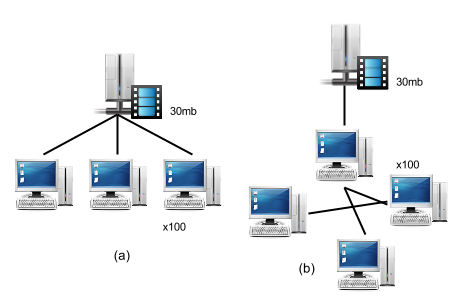
\includegraphics[scale=0.7]{gfx/conexion_video}
  \caption{Ejemplo de Conexión de Video}
  \label{conexionvideo}
\end{figure}

Otra idea podría ser que los clientes con menos recursos sirvan archivos pequeños como por ejemplo imágenes. Esto le quitaría gran cantidad de trabajo al servidor ya que una imagen significa un hilo de ejecución más que se debe crear para servir un archivo.

Uno de los objetivos es que estas comunidades se conformen de manera automática y voluntaria, esto quiere decir que un usuario instala un complemento en su navegador web y el sitio al que trata de acceder (el cual utiliza el protocolo de CWC) realiza el intercambio de manera automática sobre los archivos más relevantes que se desean mantener en caché, haciendo que éstos archivos puedan ser servidos desde la nueva ubicación dada por el nuevo miembro de la comunidad.

La cache podrá tener dos modos de operación, el primero consiste en la administración por parte del usuario, esto quiere decir que cuando el usuario accede a un contenido este queda automáticamente en la cache y el usuario puede decidir si dejarlo o eliminarlo. El segundo sería administrado por el servidor, o sea que cuando este modo se encuentra activo el servidor tendrá derecho a utilizar los recursos asignados a la caché, por lo que el servidor podrá enviar archivos que considere que deberían de estar en la caché o borrar los que no considere necesarios.

Se ampliará con mayor detalle el funcionamiento y diseño del protocolo de CWC en los siguientes capítulos.

\section{Definición del problema}

En los últimos años se ha dado un alto crecimiento en el número de usuarios de la "World Wide Web", por ejemplo a continuación se muestran las estadísticas del crecimiento de usuarios de acuerdo a el área geográfica en los últimos 10 años:

\begin{table}[h] %here h, t top, b bottom, p dedicated page on floats
\myfloatalign
\begin{tabular}{lccc} \toprule % four columns, fist left, other ones centered. 
\tableheadline{Región} & \tableheadline{2005} & \tableheadline{2010} & \tableheadline{2014}\\ \midrule
África & 2.4\% & 9.8\% & 19\% \\ 
Américas & 35.9\% & 50.5\% & 65.5\% \\
Estados Árabes & 8.3\% & 23.0\% & 40.6\% \\
Asia y Pacífico & 9.4\% & 22.5\% & 34.4\% \\
Europa & 46.3\% &	66.6\% & 74.8\% \\
\end{tabular}
\caption{Uso de Internet por Región Geográfica \citeauthor{itu:2014}.}  
\label{tab:crecimiento_internet}
\end{table}

Como se puede ver en la tabla \ref{tab:crecimiento_internet}, en casi diez años se ha duplicado o más la cantidad de usuarios de Internet, lo cual implica que se dará una mayor demanda sobre los sitios web, esto se traduce en que el dueño de un sitio web que presta un servicio deberá hacer una inversión en más recursos computacionales, como por ejemplo poder de procesamiento y ancho de banda para poder servir a sus usuarios de la mejor manera posible.

Esto quiere decir que la publicación de un sitio web con contenido de calidad no es tan trivial (se hablará en términos de contenido de calidad, ya que el contenido justificará la cantidad de usuarios que recibirá un sitio web, o sea entre mayor sea la calidad del contenido ofrecido por un sitio web para un grupo de usuarios en particular, así será la cantidad de usuarios que recibirá) ya que se deberán tomar en cuenta aspectos de crecimiento en el número de usuarios que visiten el sitio web y los requerimientos computacionales necesarios para poder prestar un servicio de calidad, acorde con los contenidos publicados.

Tomando en cuenta que realizar una publicación en Internet implica un costo para el publicador y éste se incrementa conforme aumenta el número de usuarios que soliciten los contenidos del sitio web, se podría elaborar una función de costo donde se incluyan las variables anteriormente expresadas en función de una calidad de servicio aceptable.

Este costo se traduce en que los interesados en publicar, deban de pagar por conexiones a Internet de Alta Velocidad y adquirir grandes granjas de servidores que soporten la infraestructura para hacer frente a la demanda. Es por ello que en la actualidad, solo las grandes compañías son las únicas con la capacidad de sufragar estos gastos, mediante el establecimiento de grandes caches regionales que puedan atender el tráfico generado en un área específica.

Ahora ¿Qué pasa con las pequeñas compañías, instituciones sin fines de lucro e individuos que quieren crear un sitio web con contenido de calidad y no cuentan con suficientes recursos para sufragar los gastos generados por un alto número de usuarios?. Una opción es buscar financiamiento o poner precio a sus contenidos o simplemente buscar la forma de ganar dinero mediante el bombardeo de publicidad en los sitios web, lo cual es un aspecto negativo para los usuarios.

Una vez que se han visto las necesidades de recursos computacionales para publicar contenido en Internet que es accedido por un alto número de usuarios, ¿Qué pasa con los recursos computacionales que tiene el usuario/cliente?, ¿Los recursos del cliente tienen una utilización de un 100\% en todo momento o se encuentran ociosos la mayoría del tiempo?, ya se notó que la cantidad de usuarios con acceso al World Wide Web crece enormemente, esto implica que un gran número de usuarios cuentan con una conexión a Internet con una velocidad aceptable para acceder a los contenidos de cotidianos (como videos, música, entre otros). Además también implica que cada uno de esos usuarios cuenta con una o más computadoras, las cuales obviamente cuentan con recursos computacionales aceptables para poder visualizar los contenidos ofrecidos por los sitios web, entonces se tendría la siguiente pregunta: ¿Qué sucede con todos éstos recursos de cómputo (limitado al ancho de banda, procesamiento y memoria) mientras se accede a alguna comunidad virtual, se utiliza una aplicación de ofimática, se reproduce algún contenido de multimedia en Internet o simplemente se ejecuta una aplicación de chat modo texto?  Y la respuesta es simple: se desperdician los recursos, están ociosos y están esperando a ser utilizados.

En términos de definición de la problemática, éste se encuentra compuesto por cinco partes esenciales:
\begin{enumerate}
\item Falta de recursos de quien publica contenido de calidad en Internet, esto implica un alto costo para poder atender un mayor número de clientes.
\item Un alto desperdicio de recursos en los clientes, entre estos recursos podemos citar: Ancho de Banda, Almacenamiento, Memoria y Procesamiento.
\item Una baja en la calidad del servicio conforme aumenta el número de clientes, tiempos de respuesta poco aceptables o bien se ve comprometida la continuidad del negocio. 
\item El número de usuarios en Internet se incrementa constantemente cada año, para muestra la tabla \ref{tab:crecimiento_internet}, la cual reúne el crecimiento en los últimos 10 años.
\item El problema inherente de tener un sitio con una disponibilidad del 100\%, soportando las solicitudes usuales de los clientes, las denegaciones distribuidas y las fallas en los servicios. 
\end{enumerate}

%\marginpar{¿Es posible establecer una comunidad virtual basada en una aplicación de bajo costo que utilice de una manera eficiente los recursos computacionales aportados por cada miembro y además se pueda utilizar con las aplicaciones de navegadores y servidores web utilizados actualmente?}
¿Cómo dar solución a este problema?, ¿Es posible que la solución se encuentre en una utilización eficiente de los recursos tanto del publicador cómo de los clientes?, ¿Es posible encontrar una solución de bajo costo que aproveche las causas de estos problemas para dar una solución que resuelva los problemas?, ¿Es posible el establecimiento de una comunidad virtual en la cual cada miembro de la misma, aporte un poco de recursos computacionales con el afán de mantener contenido de calidad en Internet, el cual pueda ser accedido de una forma rápida y fiable? Y aun más importante ¿Es posible establecer una comunidad virtual basada en una aplicación de bajo costo que utilice de una manera eficiente los recursos computacionales aportados por cada miembro y además se pueda utilizar con las aplicaciones de navegadores y servidores web utilizados actualmente?

\section{Justificación}

\subsection{Innovación}
%\marginpar{CWC busca establecer una comunidad en la cual cada miembro comparta un poco de sus recursos computacionales}
La Comunidad Web Caché trata de establecer una comunidad en la cual cada miembro comparta un poco de sus recursos computacionales como almacenamiento, procesamiento y ancho de banda para buscar el bien común. Esto se traduce en un incremento en la eficiencia y la velocidad del servidor web que sirve archivos.

Por otro lado, se han identificado varias problemáticas que se deben tomar en cuenta en la creación del presente proyecto y que es necesario cubrir en torno al diseño de la Comunidad Web Caché. Entre ellas se pueden mencionar:

\begin{enumerate}
\item El incremento exponencial en el número de usuarios en Internet.
\item El incremento en los recursos computacionales accesibles a los usuarios en Internet, los cuales son desperdiciados. 
\item La falta de recursos computacionales por parte de quien publica contenido de calidad en Internet, cuando aumenta el número de usuarios se vuelve un problema ya que entre más usuarios se necesitan más recursos para poder servir a estos usuarios de una manera satisfactoria.
\item La tendencia en los contenidos de moda en Internet, archivos estáticos de gran tamaño básicamente contenidos de multimedia.
\item El gran numero de comunidades con objetivos específicos que se establecen en Internet de la cual se puede tomar la decisión de formar parte.
\item La necesidad de presentar continuidad del negocio, tomando en cuenta los ataques de DDoS y tolerancia a desastres. 
\end{enumerate}
  
 
El proyecto pretende la utilización de tecnologías y productos ya establecidos, entre los cuales se tienen:

\begin{enumerate}
\item Protocolo HTTP
\item Protocolo P2P
\item Navegadores Web
\item Servidores Web
\end{enumerate}

Se podría resumir el funcionamiento de la Comunidad Web Caché como:
\begin{verse}
Quien publica contenido de calidad en Internet podrá decidir cual contenido podrá ser mantenido por la comunidad (el contenido que podrá ser mantenido por la comunidad es el que se pueda mantener en la caché, esto por el hecho de respetar el copyright). Los miembros de la comunidad podrán aportar un poco de sus recursos computacionales; es importante que ellos decidan la cantidad que aportarán. Cuando un miembro de la comunidad solicita un archivo, como un video, este será servido desde el servidor principal y desde los otros miembros de la comunidad que posean este archivo, sincronizado y previamente transferido mediante un mecanismo de P2P. Lo anterior supone que debería de incrementar la velocidad al momento de responder la solicitud, pues el archivo es seccionado y transmitido desde distintas ubicaciones, con distintos recursos y en el peor de los casos se volvería al modelo tradicional donde el archivo es distribuido desde el servidor principal. 
\end{verse}

Uno de los puntos focales del CWC es precisamente la parte comunitaria y es por ello que en el diseño se tomarán en cuenta varios conceptos propios de comunidades virtuales como: 

\begin{enumerate}
\item Aporte de recursos o participación libre: Los miembros de la comunidad decidirán qué cantidad de recursos computacionales aportaran.
\item Adhesión abierta: Puedo decidir formar parte de la comunidad o no.
\item Respeto por los contenidos privados: Se respeta el Copyright. Quien publica estos contenidos, podrá decidir si pueden ser mantenidos por la comunidad o no.
\item Bien común: los contenidos deben ser servidos de manera rápida y eficiente.
\item Apoyo: Si alguno de los miembros de la comunidad falla otro podrá tomar su lugar (tolerancia a fallos).
\end{enumerate}

En general, el CWC busca el establecimiento de una comunidad cooperativa sobre Internet utilizando los navegadores y servidores web actuales, y se diferencia de otras soluciones ya existentes. Por ejemplo, los Proxys buscan mejorar el rendimiento sobre una red de área local. 

Por otro lado, uno de los modelos más parecidos a CWC son los Proxy Federados, mejor conocidos como "Cooperative Web Caching". Éstos buscan tener un conjunto de servidores proxy que se comuniquen y que compartan los contenidos que tienen en cache sobre cualquier tipo de red, podrían utilizar en una WAN o incluso en Internet. Pero en comparación a éste último, en el CWC cualquier usuario puede formar parte de la comunidad, sin necesidad de tener que configurar un Proxy dedicado.


\subsection{Impacto}


El proyecto impactará tanto al publicador de contenido de calidad en Internet, así como a los usuarios, en los siguientes aspectos:

\paragraph{Publicador}


\begin{itemize}
\item Conforme el número de miembros de la comunidad crezca, se podrá experimentar menos carga en los servidores, por consiguiente se podrán servir muchos más usuarios.
\end{itemize}
 

\paragraph{Usuario}
\begin{itemize}
\item Conforme el número de miembros de la comunidad crezca, se podrá experimentar una utilización más eficiente de sus recursos computacionales, una mejora en los tiempos de respuesta cuando se hace una petición a un servidor web y una mayor tolerancia a fallos, dándole continuidad al negocio. 
\end{itemize}

\subsection{Profundidad}
En relación a los temas que cubrirá el presente proyecto son:
\begin{itemize}
\item Se realizará una investigación del estado del arte, en relación a los protocolos, algoritmos y mecanismo que ayuden a soportar el diseño del CWC.
\item Se realizará un levantamiento de requerimientos relacionado a las necesidades entorno a CWC.
\item Se creará un diseño completo de la implementación de CWC.
\item Se realizarán modelos que prueben el rendimiento y costos de la CWC.
\end{itemize}

Quedan fuera del alcance de este proyecto:

\begin{itemize}
\item La aplicación del protocolo de CWC en un ambiente de páginas dinámicas.
\item La aplicación del protocolo de CWC en un ambiente de flujo de video o sonido.
\item La seguridad en general, tanto del servidor como del cliente. No se especificó ningún mecanismo que permita la comprobación y la autenticidad de los elementos.
\end{itemize}

\section{Hipótesis}
El desarrollo de una caché web distribuida que permita compartir de manera transparente y eficiente los recursos computacionales distribuidos ofrecidos colaborativamente mediante una comunidad de servidores, tendrá un impacto positivo en el bajar los costos y mejorar la continuidad del negocio para las comunidades virtuales.

\section{Objetivos}
\subsection{Objetivo Principal}
Desarrollar una caché web distribuida que permita compartir de manera transparente y eficiente los recursos computacionales distribuidos ofrecidos colaborativamente mediante una comunidad de servidores.

\subsection{Objetivos Específicos}
\begin{itemize}
\item Compilar y comparar trabajos relevantes relacionados con sistemas distribuidos
\item Examinar las oportunidades de mejoramiento estratégico de las plataformas existentes.
\item Determinar los requerimientos de la caché web distribuida basada en HTTP.
\item Diseñar una arquitectura de una caché web distribuida bajo un conjunto de principios tales como: transparencia de ubicación de los recursos, solución de bajo costo y calidad de servicio.
\item Desarrollar un prototipo de la caché web distribuida.
\item Analizar el rendimiento de velocidad y el costo del entorno de CWC.
\end{itemize}

\section{Alcances}

\begin{itemize}
\item Investigación del funcionamiento de Protocolos P2P y HTTP.
\item Investigación de los diferentes modelos de caching existentes con el fin de identificar sus características, arquitectura, funcionamiento, debilidades y fortalezas. Esto ayudará en una etapa posterior para realizar el diseño de la Comunidad Web Caché.
\item Investigación sobre el establecimiento de comunidades virtuales y las implicaciones de estas.
\item Investigación  a soluciones que utilicen los diferentes modelos de web caching, esto permitirá tener un punto de comparación para nuestros modelo y establecerá los umbrales a mejorar.
\item Investigación de modelos de consistencia.
\item Elaboración del diseño del CWC el análisis de las investigaciones previas. Este modelo se limitará únicamente a contenido estático y no se desarrollará el diseño para la compatiblidad de contenido dinámico y contenidos de flujo de video o sonido, los cuales implican modelos de consistencia mucho más complejos, además de algoritmos de reemplazo y muchas otras implicaciones de diseño que necesitan de una investigación aún mayor.
\item Elaboración de prototipo de sistema para compartir archivos de manera distribuida tomando en cuenta ciertas partes del diseño. Este prototipo pretende convertirse en la base para el desarrollo del CWC.
\end{itemize}

\section{Entregables}
\begin{enumerate}
\item Informe investigación funcionamiento de protocolo HTTP.
\item Informe investigación funcionamiento de protocolo P2P.
\item Informe investigación de modelos de Web Caché existentes.
\item Informe investigación sobre comunidades virtuales.
\item Informe investigación de aplicaciones que utilicen los diferentes modelos de Web Caché.
\item Informe investigación de modelos de consistencia.
\item Documento de requerimientos de Comunidad Web Caché.
\item Prototipo de CWC Cliente.
\item Prototipo de CWC Server.
\item Análisis de rendimiento de velocidad del entorno de CWC.
\item Análisis de costos del Entorno de CWC.
\end{enumerate}  

%---------------------------------------------------------------------------------------- % Chapter 1 - Introducción

\ctparttext{En los siguientes capítulos se aclararán temas relacionados a los protocolos utilizados por CWC, como lo son HTTP y P2P. Además establecerán todas aquellas definiciones necesarias para el desarrollo de la presente investigación.} % Text on the Part 1 page describing  the content in Part 1

\part{Marco Teórico} \label{part:marco_teorico} % First part of the thesis
% Chapter 2

\chapter{Protocolo HTTP} % Chapter title

\label{ch:protocolo_http} % For referencing the chapter elsewhere, use \autoref{ch:protocolo_http} 

%----------------------------------------------------------------------------------------

%\lipsum[1]

%----------------------------------------------------------------------------------------

\section{¿Cómo trabaja?}

El protocolo HTTP es un protocolo petición/respuesta. Un cliente envía una petición al servidor en la forma de un método de petición, URI, versión de protocolo, seguido de un mensaje estilo-
MIME conteniendo los modificadores de la petición, información del cliente y posiblemente el contenido del cuerpo sobre una conexión con el servidor, el servidor resuelve con un mensaje de estatus, incluyendo la versión del protocolo del mensaje y el código de error o éxito, seguido de un mensaje estilo-MIME que contiene la información del servidor, la meta-información de la entidad y posiblemente el contenido del cuerpo de la entidad.
La conexión más simple sería cuando el agente de usuario realice una conexión directa con el servidor de origen. Un ejemplo de la conexión de una petición se muestra en la figura \ref{conexionhttp}.

\begin{figure}[h]
  \centering
    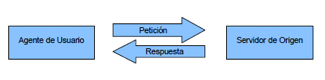
\includegraphics[scale=0.75]{gfx/conexion_http}
  \caption{Conexión HTTP}
  \label{conexionhttp}
\end{figure}


En conexiones más complejas pueden intervenir uno o más intermediarios, como lo pueden ser:

  \begin{itemize}
     \item Proxies que son agentes de reenvío, este recibe peticiones para un URI en su forma absoluta, sobre escribe toda o parte del mensaje y reenvía las peticiones re-formateadas hacia el servidor identificado por la URI.
     \item Gateway es un agente de recepción, actuando como una capa sobre otros servidores y si es necesario traduce la petición al protocolo del servidor subyacente.
     \item Túnel: Actúa como un punto de transmisión entre dos conexiones sin cambiar el mensaje, los túneles son usados cuando la conexión pasa a través de un intermediario (como un firewall) aún cuando el intermediario no entiende los contenidos del mensaje.
  \end{itemize}


%------------------------------------------------
\section{Mensajes HTTP}

\begin{description}
\item[Tipos de Mensajes:] 

Los tipos de mensajes HTTP son de petición de un cliente hacia el servidor y de respuesta de un servidor hacia el cliente.

\begin{lstlisting}[caption={Tipos de mensajes HTTP},label={lst:mensajes_http}]
"HTTP-message = Request | Response ; HTTP/1.1 messages"
\end{lstlisting}

Los mensajes Request y Response utilizan la forma genérica de mensajes, definido en RFC822 para transferencia de mensajes. Ambos mensajes consisten una línea de inicio, uno o más valores de encabezado, una línea vacía que indica el final de los valores de encabezado y posiblemente un cuerpo del mensaje \cite{rfc2616}.

A continuación se describirán con más detalle los mensajes mínimos necesarios para establecer una comunicación HTTP: 

\item[Encabezados del Mensaje:] 
Los valores HTTP, los cuales incluyen general-header, request-header, response-header y entity-header, siguen el mismo formato genérico del RFC822. Cada campo del encabezado consiste de un nombre seguido por “:” y un valor. Los nombres de campos son case-insensitive, el valor se puede extender múltiples líneas y el orden en que se reciben de los campos del header no es significativo \cite{rfc2616}.

\item[Cuerpo del Mensaje:] 

El cuerpo del mensaje de un mensaje HTTP es utilizado para trasportar el cuerpo de la entidad asociado con la respuesta o la petición. El cuerpo del mensaje difiere del cuerpo de la entidad solo cuando una codificación de transferencia ha sido aplicada. “message-body = entity-body | entity-body codificado”  
El campo Transfer-Encoding debe ser utilizado para indicar cualquier codificación de transferencia aplicada por una aplicación para asegurar la transferencia adecuada del mensaje. Transfer-Encoding es una propiedad del mensaje no de la entidad \cite{rfc2616}.

\item[Largo del Mensaje:] 

El transfer-length de un mensaje es el largo del cuerpo del mensaje a como este aparece en el mensaje, sin que se haya aplicado ningún filtro. Cuando el cuerpo del mensaje es incluido con un mensaje, el transfer-length de ese cuerpo es determinado por uno de \cite{rfc2616}: 
\begin{itemize}

\item Cualquier mensaje de respuesta que no incluya cuerpo del mensaje como las repuestas de estado 1xx, 204 y 304 son siempre terminadas con la primer línea vacía después de los campos de encabezado presentes en el mensaje.
\item Si un campo de Transfer-Encoding se encuentra especificado y tiene cualquier valor diferente a “Identity”, entonces el transfer-length está determinado por el uso de "chunked" transfer-coding, a menos que el mensaje se terminara por que se cerró la conexión.
\item Si un campo Content-Length se encuentra presente, su valor decimal en octetos representa el entity-length y transfer-length. Content-Length no se debe enviar si los dos anteriores no son iguales. 
\item Si el mensaje utiliza el tipo de media "multipart/byteranges" y el largo de trasferencia no está especificado, entonces este tipo de media determina el transfer-length. Este tipo de media no debe ser utilizado a menos que quien envía conozca que el recipiente lo puede parsear.
\item Por un cierre de conexión por parte del servidor

\end{itemize}


\end{description}

\section{Petición}
Un mensaje de petición de un cliente hacia un servidor incluye, en la primera línea de ese mensaje, el método a ser aplicado al recurso, el identificador del recurso y la versión del protocolo en uso \cite{rfc2616}.

\begin{lstlisting}[caption={Mensaje de petición},label={lst:mensajes_peticion}]
"Request = Request-Line * (( general-header |  \\
 request-header | entity-header ) CRLF) \\  
 CRLF
 [message-body]"
\end{lstlisting}

\begin{description}
\item [Línea de Petición: ]
La línea de petición inicia con un token de método, seguido por la URI que se está pidiendo y la versión del protocolo y terminando con CRLF (retorno de carro y cambio de línea). Los elementos son separados por caracteres SP \cite{rfc2616}.

\begin{lstlisting}[caption={Línea de petición},label={lst:linea_peticion}]
"Request-Line = Method SP Request-URI SP \\ 
HTTP-Version CRLF"
\end{lstlisting}

\item[Método] 
El token de método indica el método a ser aplicado al recurso identificado por la URI-pedida. El método es case-sensitive. El listado de los métodos del protocolo HTTP se puede observar en la tabla \ref{tab:metodos_http}.

\begin{table}
\myfloatalign
\begin{tabularx}{\textwidth}{lp{8cm}} \toprule
\tableheadline{Método} & \tableheadline{Descripción} \\ \midrule
OPTIONS & Representa una solicitud de información acerca de las opciones de comunicación disponibles en la cadena de Petición/Respuesta identificada por el URI-pedida. \\
GET & Significa que se recupere cualquier información (en la forma de entidad) que es identificada por la URIpedida.  \\
HEAD & Es idéntica a GET con la excepción de que el servidor no retornara en cuerpo del mensaje en la respuesta. \\
POST & Se utiliza para solicitar que el servidor original acepte la entidad envuelta en la petición como un nuevo subordinado del recurso identificado por el URIpedida en la línea de petición. \\
PUT & Solicita que la entidad envuelta sea almacenada bajo el URI-perdida suplida.  \\
DELETE & Solicita que el servidor original borre el recurso identificado por el URI-pedida \\
TRACE & Es utilizada para invocar un remoto, de nivel de aplicación loop- back del mensaje de petición.  \\
CONNECT & Se utiliza con proxies que pueden dinámicamente  cambiarse para ser un túnel. \\
extension-method & Definidos por alguna aplicación. \\
\end{tabularx}
\caption[Métodos de HTTP]{Métodos de HTTP \citeauthor{Tanenbaum:2011}.}  
\label{tab:metodos_http}
\end{table}

\item[URI-Solicitada]
La URI-Solicitada es un identificador uniforme de recurso (URI) e identifica el recurso sobre el cual se va a aplicar el mensaje de petición.

\begin{lstlisting}[caption={URI-Solicitada},label={lst:uri_solicitada}]
"Request-URI = "*" | absoluteURI | abs_path | authority"
\end{lstlisting}

Las opciones del URI-pedida dependen de la naturaleza de la petición. El asterisco significa que la petición no aplica a ningún recurso en particular, pero al servidor en sí mismo y solo es permitido cuando el método utilizado no necesariamente aplica a un recurso \cite{rfc2616}.

\item[El recurso identificado por una petición]

Para extraer el identificador de recurso por una petición en Internet es determinado mediante el proceso de examinar ambos URI-pedida y el campo del encabezado HOST.
Un servidor de origen que no diferencie recursos de acuerdo en el host solicitado debe utilizar las siguientes reglas para identificar el recurso pedido \cite{rfc2616}:
\begin{enumerate}
\item Si URI-pedida es un URI absoluta, el HOST es parte de URI-pedida. Cualquier campo de encabezado HOST debe ser ignorado.
\item Si URI-pedida no es una URI absoluta y la petición incluye un campo de encabezado HOST, el HOST es determinado por el campo HOST de la petición. 
\item Si el HOST identificado por las reglas 1 y 2 no es un HOST valido en el servidor entonces el servidor deberá devolver la respuesta 400 Bad Request.
\end{enumerate}

\item[Campos de encabezado de una Petición]

El encabezado de la petición permite a el cliente pasar información adicional acerca de la petición y acerca del cliente al servidor. Estos campos actúan como modificadores de la petición, con semántica equivalente a los parámetros en la invocación de métodos en los lenguajes de programación. Un ejemplo de los campos de encabezado más importantes se pueden ver en la tabla \ref{tab:encabezado_peticion}.

\begin{table}
\myfloatalign
\begin{tabularx}{\textwidth}{lp{8cm}} \toprule
\tableheadline{Método} & \tableheadline{Descripción} \\ \midrule
Accept & Se utiliza para especificar ciertos tipos de media que son aceptables por la respuesta. \\
Accept-Charset & Se utiliza para indicar cuales CHARSETS son aceptables en la respuesta.  \\
Accept-Encoding & Similar a ACCEPT pero limita los content-encodings aceptables en la respuesta. \\
Accept-Language & Similar a ACCEPT pero con la diferencia que restringe el conjunto de lenguajes que son preferidos como respuesta a la petición. \\
Authorization & Se utiliza cuando el agente de usuario quiere identificarse con él con el servidor. Se envían las credenciales. \\
Cache-Control & Se utiliza para especificar directivas que deben ser  obedecidas por todos los mecanismos de cache a lo largo de la cadena de Petición/Respuesta. \\
Cookie & Muestra la cookie establecida privamente que se regresa al servidor. \\
Host & Contiene el nombre de DNS del servidor. \\
User-Agent & Contiene la información sobre el navegador y su plataforma. \\
Referer & El URL anterior desde el cual provino la solicitud. \\
Set-Cookie & La cookie que debe guardar el cliente. \\
Server & Información sobre el servidor web. \\

\end{tabularx}
\caption[Métodos de Petición]{Métodos de Petición \citeauthor{Tanenbaum:2011}.}  
\label{tab:encabezado_peticion}
\end{table}


\end{description}

\section{Respuesta}
Después de recibir el interpretar un mensaje de petición, el servidor responde con un mensaje de respuesta HTTP.

\begin{lstlisting}[caption={Mensaje de respuesta HTTP},label={lst:respuesta_http}]
"Response = Status-Line *(( general-header |  \\
response-header | entity-header ) CRLF) 
CRLF 
[message-body ]"
\end{lstlisting}

\begin{description}

\item[Línea de Estado: ]
La primera línea de un mensaje de respuesta es Status-Line, la cual se encuentra conformada por una versión de protocolo seguida por un código numérico de estatus y su frase de texto asociada, con cada elemento separado por caracteres SP \cite{rfc2616}.

\begin{lstlisting}[caption={Línea de Estado},label={lst:linea_estado}]
"Status-Line = HTTP-Version SP Status-Code \\ 
SP Reason-Phrase CRLF"
\end{lstlisting}

\item[Código de Estado y Frase: ]
El código de estado es un código de resultado de 3 dígitos que indica el intento de entender y satisfacer la petición. Esos códigos ya se encuentran definidos. La frase intenta dar una corta descripción textual del Código de estado \cite{rfc2616}.

\item[Encabezado de Respuesta: ]
Los campos del encabezado de respuesta permiten al servidor pasar información adicional acerca de la respuesta que no pueden ser colocadas en la Status-Line. Estos campos del encabezado dan información acerca del servidor y acerca de futuros accesos al recurso identificado por la URI-Pedida \cite{rfc2616}.
\end{description} % Chapter 2 HTTP
% Chapter X

\chapter{Protoloco P2P} % Chapter title

\label{ch:protocolo_p2p} % For referencing the chapter elsewhere, use \autoref{ch:name} 

Una red peer-to-peer (P2P) o red de pares, es una red de computadoras en la que todos o algunos aspectos de ésta funcionan sin clientes ni servidores fijos, sino una serie de nodos que se comportan como iguales entre sí. Es decir, actúan simultáneamente como clientes y servidores respecto a los demás nodos de la red.\cite{wiki_p2p}

Las redes peer-to-peer aprovechan, administran y optimizan el uso del ancho de banda de los demás usuarios de la red por medio de la conectividad entre los mismos, obteniendo más rendimiento en las conexiones y transferencias que con algunos métodos centralizados convencionales, donde una cantidad relativamente pequeña de servidores provee el total del ancho de banda y recursos compartidos para un servicio o aplicación.
Alfredo F. nos dice que de forma simple puede verse como la comunicación entre pares o iguales utilizando un sistema de intercambio \cite{bordignon:2005}.

Los sistemas compañero a compañero (o P2P por sus siglas en inglés) permiten que computadoras de usuario final se conecten directamente para formar comunidades, cuya finalidad sea el compartir recursos y servicios computacionales. En este modelo, se toma ventaja de recursos existentes en los extremos de la red, tales como tiempo de CPU y espacio de almacenamiento. Las primeras aplicaciones  emergentes se orientaban a compartir archivos y a la mensajería \cite{bordignon:2005}.


%----------------------------------------------------------------------------------------

\section{Clasificación}

\subsection{Directorio Centralizado}

Esta primera visión se puso en práctica para el año 1997 con la red Napster. Bajo este modelo los clientes o peers realizan el descubrimiento y búsqueda de los otros miembros mediante un servidor central, luego el mismo servidor se encarga de negocia la conexión entre ambos clientes.

Este tipo de red P2P se basa en una arquitectura monolítica en la que todas las transacciones se hacen a través de un único servidor que sirve de punto de enlace entre dos nodos y que, a la vez, almacena y distribuye los nodos donde se almacenan los contenidos. Poseen una administración muy dinámica y una disposición más permanente de contenido. Sin embargo, está muy limitada en la privacidad de los usuarios y en la falta de escalabilidad de un sólo servidor, además de ofrecer problemas en puntos únicos de fallo, situaciones legales y enormes costos en el mantenimiento así como el consumo de ancho de banda. \cite{wiki_p2p}

El principal problema presentado en este modelo es que el servidor P2P Central es un posible punto de quiebre que pueda atentar contra la estabilidad de la red.

\begin{figure}[h]
  \centering
    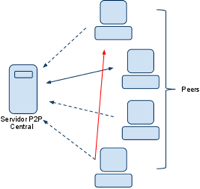
\includegraphics[scale=1]{gfx/p2p_central}
  \caption{Directorio Centralizado}
  \label{conexionhttp}
\end{figure}

%------------------------------------------------

\subsection{Solución Distribuida}

Las redes P2P de este tipo son las más comunes, siendo las más versátiles al no requerir de un gestiona miento central de ningún tipo, lo que permite una reducción de la necesidad de usar un servidor central, por lo que se opta por los mismos usuarios como nodos de esas conexiones y también como almacenistas de esa información. En otras palabras, todas las comunicaciones son directamente de usuario a usuario con ayuda de un nodo (que es otro usuario) quien permite enlazar esas comunicaciones \cite{wiki_p2p}.

\begin{figure}[h]
  \centering
    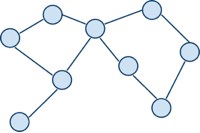
\includegraphics[scale=1]{gfx/p2p_distribuido}
  \caption{Solución Distribuida}
  \label{conexionhttp}
\end{figure}

%------------------------------------------------

\subsection{Directorio Descentralizado }

En este tipo de red, se puede observar la interacción entre un servidor central que sirve como hub y administra los recursos de banda ancha, enrutamientos y comunicación entre nodos pero sin saber la identidad de cada nodo y sin almacenar información alguna, por lo que el servidor no comparte archivos de ningún tipo a ningún nodo. Tiene la peculiaridad de funcionar (en algunos casos como en Torrent) de ambas maneras, es decir, puede incorporar más de un servidor que gestione los recursos compartidos, pero también en caso de que el o los servidores que gestionan todo caigan, el grupo de nodos sigue en contacto a través de una conexión directa entre ellos mismos con lo que es posible seguir compartiendo y descargando más información en ausencia de los servidores \cite{wiki_p2p}.

\begin{figure}[h]
  \centering
    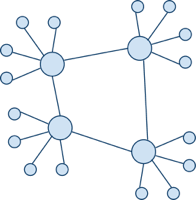
\includegraphics[scale=1]{gfx/p2p_dir_centralizado}
  \caption{Directorio Descentralizado}
  \label{conexionhttp}
\end{figure}

%----------------------------------------------------------------------------------------

\section{Mecanismos de búsqueda en Redes P2P}

\begin{description}
\item[Centralizados: ]
Un repositorio central almacena un índice de todos los recursos en la red, junto con la localización de dichos recursos (qué nodos los ofrecen). Todos los miembros de la red registran sus recursos y dirigen sus búsquedas a este repositorio. Un ejemplo es la red Napster. En realidad, a los sistemas de este tipo no se les considera como P2P puros, ya que ese repositorio es un servicio centralizado, con los inconvenientes típicos: representa un punto único de fallo, y compromete la escalabilidad del sistema.

\item[Descentralizados: ]
No existe ningún repositorio centralizado. Para encontrar un recurso, los nodos lanzan mensajes de búsqueda que son encaminados por la red. Las redes descentralizadas son clasificadas a su vez en: Redes no estructuradas y Redes estructuradas.

\item[Redes Estructuradas: ]
Las redes estructuradas tienen importantes ventajas. Proporcionan un mecanismo determinista de localización, de tal forma que se asegura que un recurso será encontrado siempre que esté en la red. Además, los mensajes de búsqueda son encaminados de forma eficiente, de tal forma que el recurso es encontrado en $O(\log n)$ saltos, donde $n$ es el tamaño de la red.

\end{description} % Chapter 3 P2P
% Chapter X

\chapter{Modelos de Web Caché} % Chapter title

\label{ch:modelos_web_caching} % For referencing the chapter elsewhere, use \autoref{ch:name} 

El web caché no es un concepto nuevo. Este tema ya se ha estudiado y también ha sido objeto de numerosos papers, artículos y tesis. Por otro lado el concepto de caché web distribuida es un poco más nuevo pero también suma bastantes proyectos entorno a él.

Como primer acercamiento, es necesario definir el el significado de caché web (en ocasiones también llamado proxy) \cite{wiki_cacheweb}:

"Se llama caché web a la caché que almacena documentos web (es decir, páginas, imágenes, entre otros) para reducir el ancho de banda consumido, la carga de los servidores y el retardo en la descarga. Un caché web almacena copias de los documentos que pasan por él, de forma que subsiguientes peticiones pueden ser respondidas por el propio caché, si se cumplen ciertas condiciones." 

En resumen, se podría entender una caché web como una forma de almacenar temporalmente documentos que son concurrentemente solicitado con el fin de reducir el ancho de banda saliente. Por otro lado, la presente investigación se centra en modelos que comparten dinámicamente éstos documentos. 

Un concepto muy parecido es el de caché web cooperativo. Según Rowstron A. \cite{rowstron:2001} mediante esta técnica, el almacenamiento dedicado a la caché de una serie de servidores-proxy adyacentes se gestiona conjuntamente como si se tratase de una única cache distribuida. Las políticas de gestión de esta cache se realiza teniendo en cuenta el estado y los contenidos de todos los servidores-proxy que la componen. Por ejemplo, las políticas de reemplazo en la cache cooperativa tendrán en cuenta las estadísticas de acceso en todos los servidores-proxy cooperantes.

El caché web cooperativo permite incrementar considerablemente el tamaño de la caché, pero a costa de
reducir la probabilidad de acierto local. Bajo éste esquema, un único servidor-proxy no dispone de los contenidos más populares, provocando un aumento del porcentaje de peticiones que se tienen que servir remotamente desde los otros servidores que componen la cache ó desde el servidor principal.

Basado en la investigación del estado del arte, se han podido identificar proyectos que giran alrededor de la presente tesis. Entre ellos están: CoralCDN \cite{freedman:2004}, Transparent Distributed Web Caching \cite{liang:2001}, Dalesa \cite{wathsala:2009} y Squirrel \cite{rowstron:2001}.


%----------------------------------------------------------------------------------------

\section{Web Caching mediante Proxy}

%------------------------------------------------

\subsection{Proxy Simple}

Primero se mostrará el modelo tradicional de cliente-servidor. Bajo este modelo el cliente tiene una conexión directa con el servidor y no existe caché en medio, por lo que en dicha conexión se obtienen los servicios bajo demanda, haciendo uso únicamente del caché local del explorador web.

\begin{figure}[h]
  \centering
    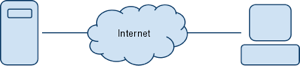
\includegraphics[scale=1]{gfx/proxy_simple_1}
  \caption{Conexión Directa}
  \label{proxy_simple_1}		
\end{figure}

La siguiente figura \ref{proxy_simple_2} muestra el típico modelo de proxy, donde existe un servidor central por el cual los clientes transitan y le solicitan el recurso deseado. El servidor proxy descarga el recurso solicitado, lo almacena en su caché y por último lo reenvía al solicitante. Si otro cliente solicitara el mismo recurso, el servidor le respondería con el recurso almacenado localmente (si la caché haya caducado aún).

\begin{figure}[h]
  \centering
    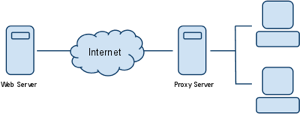
\includegraphics[scale=1]{gfx/proxy_simple_2}
  \caption{Proxy Simple}
  \label{proxy_simple_2}
\end{figure}

%------------------------------------------------

\subsection{Proxy Jerárquico}

La figura \ref{proxy_jerarquico} muestra el modelo de proxy jerárquico o también conocido como web caché cooperativo. En este modelo se tienen servidores proxy ubicados de una manera jerárquica en una Red de área local. Cuando un cliente solicita un recurso, éste lo hace a su proxy jerárquicamente más cercano. Si dicho servidor posee los recursos éste se lo reenvía al cliente. En caso que no posee el recurso, el proxy le reenvía la solicitud de su cliente al servidor proxy de nivel superior. Si el servidor de nivel superior posee el recurso lo reenvía al servidor proxy que solicitó el recurso, éste último se deja una copia en su caché local y reenvía el recurso al cliente original.

\begin{figure}[h]
  \centering
    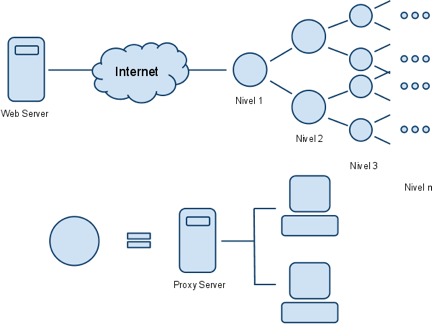
\includegraphics[scale=0.75]{gfx/proxy_jerarquico}
  \caption{Proxy Jerárquico}
  \label{proxy_jerarquico}
\end{figure}

%----------------------------------------------------------------------------------------

\subsection{Proxy Descentralizado}

Bajo este modelo se encuentran los proyectos de Squirrel y Dalesa. Estos proyectos intentan utilizar los conceptos de P2P para implementar y compartir una cache distribuida a través de una LAN. Como se muestra en la figura \ref{proxy_descentralizado}. Cada computadora forma parte del proxy descentralizado, y utilizando un software creado por los respectivos participantes del proyecto, pueden compartir la cache. Este modelo es el que más se acerca al modelo que se propone como tesis aunque todavía dista en ciertas características.

\begin{figure}[h]
  \centering
    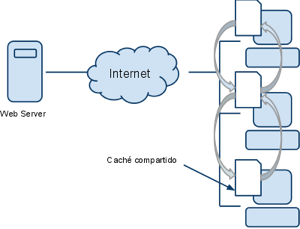
\includegraphics[scale=1]{gfx/proxy_descentralizado}
  \caption{Proxy Descentralizado}
  \label{proxy_descentralizado}
\end{figure}

\section{Redes CDN}
Una red de distribución de contenidos es una red de equipos que opera de forma transparente para entregar contenido de sus clientes cumpliendo principalmente alguno de los siguientes objetivos:
\begin{enumerate}
\item Escalabilidad
\item Coste
\item Eficiencia
\end{enumerate}

Haciendo una definición más amplia una Red CDN es un sistema de computadoras el cual contiene copias de datos, ubicados en varios puntos de la red para así maximizar el ancho de banda para el acceso de los datos desde los clientes a través de la red. Un cliente accede una copia de los datos, la más cercana, contrario al concepto de que todos los clientes accedan al mismo servidor central provocando un cuello de botella en el servidor \cite{wiki_cdn}.

El contenido puede incluir objetos web, objetos descargables (archivos de medios, software, documentos, entre otros), aplicaciones, media streams en tiempo real, y otros componentes.

En la siguiente figura se puede observar el funcionamiento de una Red CDN distribuida a través de Internet.

\begin{figure}[h]
  \centering
    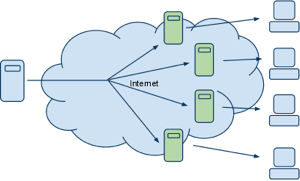
\includegraphics[scale=1]{gfx/redes_cdn}
  \caption{Red CDN}
  \label{conexionhttp}
\end{figure}
 % Chapter 4 Modelos de Web Caching
% Chapter X

\chapter{Modelos de Cosistencia} % Chapter title

\label{ch:modelos_consistencia} % For referencing the chapter elsewhere, use \autoref{ch:name}

Un requerimiento importante en los sistemas distribuidos es la replicación de datos, lo datos por lo general se replican para mejorar fiabilidad y incrementar el rendimiento, uno de los problemas más importantes es, mantener todas las réplicas consistentes, esto quiere decir que cuando una copia se actualiza, necesitamos asegurar que las otras copias se actualizan también.  

%----------------------------------------------------------------------------------------

\section{Razones para Replicar}

\begin{enumerate}
\item Los datos se replican para incrementar la fiabilidad del sistema, esto quiere decir que si el sistema ha sido replicado este puede seguir trabajando después de alguno de sus nodos falle, mediante el cambio a uno que si funcione. Al mantener muchas copias es posible proporcionar una mejor protección contra datos corruptos. 
\item Los datos se replican para incrementar el rendimiento, es importante cuando un sistema distribuido necesita ser escalado en números y áreas geográficas. En el caso de números, cuando un sistema necesita procesar mucha información, este se escala agregando otro nodo al sistema y replicando los datos, para dividir el trabajo. En el caso de área geográfica se coloca una copia cerca del proceso que lo necesita, para reducir el tiempo de acceso a los datos.

\end{enumerate}

%------------------------------------------------

\section{Modelos de Consistencia sin Sincronización}

\begin{description}

\item[Linearizability o Consistencia Estricta: ]
Según Herlihy M. \cite{herlihy} linearizability es la condición correcta para objetos concurrentes. Las operaciones write que se ejecutan en cualquiera de los sitios de un sistema, se ejecutan simultáneamente en todas las copias de los datos, osea es la condición ideal siempre las copias son coherentes. 
En pocas palabras es la consistencia más estricta, esta establece que cualquier operación de lectura en el sistema, debe devolver el valor con la última actualización antes de realizar la lectura. Lo cual quiere decir que el tiempo máximo para propagar una actualización al resto de sitios en el sistema es cero. 

\item[Consistencia Secuencial: ]
Es un modelo de consistencia un poco más débil, que la consistencia estricta. Básicamente Lamport \cite{lamport:1979} lo define mediante:

"El resultado de cualquier ejecución es el mismo que si las operaciones de todos los procesos fueran ejecutadas en algún orden secuencial, y las operaciones de cada proceso individual aparecen en esta secuencia en el orden especificado por su programa". 

La consistencia secuencial no garantiza que una operación de lectura devuelva el valor escrito por otro proceso. Lo único que asegura es que todos los sitios vean todas las operaciones en el mismo orden.

\item[Consistencia Causal: ]
Según Reynal M. \cite{raynal:1995}, en un sistema se da consistencia causal si las escrituras parcialmente relacionadas de forma causal (sobre el mismo objeto concurrente) son vistas por todos los procesos en el mismo orden, las escrituras concurrentes pueden ser vistas en un orden diferente en maquinas diferentes.

Este modelo es aun más débil que la consistencia secuencial \cite{ahamad:1991}, la cual requiere que todos sitios vean las escrituras en el mismo orden.

Cuando un sitio realiza una lectura seguida de una escritura, aun en diferentes objetos concurrentes, se dice que la primera operación esta causalmente ordenada antes que la segunda, debido a que el valor almacenado por la escritura puede haber sido dependiente del resultado de la lectura. De manera similar una operación de lectura puede estar causalmente ordenada después de una escritura previa en el mismo objeto concurrente que almacena lo que fue leído. De la misma manera dos operaciones de escritura en el mismo sitio se encuentran causalmente ordenadas en el mismo orden que fueron realizadas. 

Si existen operaciones que no están causalmente relacionadas se dice que son concurrentes.

\item[Consistencia PRAM: ]
Lipton y Sandberg \cite{lipton:1988} definieron el modelo de cosistencia Pipelined RAM (PRAM) y comúnmente conocido como Consistencia FIFO. Este modelo es aun más débil que la consistencia causal, esta consiste en eliminar el requisito de que las operaciones relacionadas se vean en orden por parte de todos los sitios en un sistema. Para esto las escrituras por un sitio son recibidas por otros procesos en el orden en que son realizadas, pero las escrituras de sitios diferentes pueden verse en un orden distinto en sitios diferentes \cite{mosberger:1993}.

Este tipo de consistencia es fácil de implementar, ya que no existe garantía del orden en que los diferentes sitios vean las escrituras, más que dos o más escrituras por parte de un proceso llegan en orden, como si estuvieran entubadas. Remontándonos a la definición de consistencia causal, podemos decir que en consistencia FIFO todas las escrituras y lecturas locales (realizadas en el mismo sitio) están causalmente relacionadas, mientras que todas las que suceden en sitios diferentes son concurrentes \cite{mosberger:1993}.


\end{description}

%------------------------------------------------

\section{Modelos de Consistencia con Sincronización}

\begin{description}

\item[Consistencia Débil:]

La consistencia débil utiliza variables de sincronización para propagar las escrituras a todo el sistema, mediante esto una operación de escritura en un sitio, tomará un candado el cual evitará que otros puedan leer o escribir hasta que la operación termine y se propague al resto de los sitios que conforman el sistema. A este mecanismo se le llama exclusión mutua.

El modelo tiene las siguientes condiciones \cite{mosberger:1993}:

\begin{itemize}
\item Los accesos a las variables de sincronización son secuencialmente consistentes.
\item No se permite ingresar a una variable de sincronización hasta que todas las operaciones de escritura hayan terminado en el resto de los sitios.
\item No se permite realizar un acceso a los datos (operaciones de lectura y escritura) hasta realizar todos los accesos a las variables de sincronización. 
\end{itemize}


\item[Consistencia Release:]
Es muy parecida a la Consistencia Débil \cite{mosberger:1993}, lo que hace es dar solución a un problema de rendimientos que tiene ésta. Cuando se accede a una variable de sincronización, el objeto concurrente no sabe si se debe a que el sitio ha terminado de escribir en el objeto concurrente o está a punto de iniciar su lectura. Para una implementación más eficiente que la Consistencia Débil, se crean dos variables de sincronización que diferencien estos casos. Estas operaciones se llaman release y acquire \cite{Gharachorloo1990}, antes de realizar una operación de escritura a un objeto concurrente un sitio debe adquirir el objeto mediante la operación acquire y más tarde liberarlo mediante release.

Para contar con consistencia release se debe cumplir:

\begin{itemize}
\item Antes de realizar una operación  a un objeto concurrente, deben terminar con éxito todas las adquisiciones anteriores del sitio en cuestión.
\item Antes de realizar un release, se deben terminar todas las escrituras y lectura del sitio.
\item Los accesos a release y acquire deben de ser consistentes con el procesador.
\end{itemize}


\item[Consistencia de Entrada: ]
El modelo de Consistencia de Entrada es aún más débil que el de Consistencia Release \cite{bershad:1991}. Utiliza las mismas operaciones de sincronización mencionadas anteriormente acquire y release. La diferencia radica en que requiere que cada objeto concurrente se asocie con alguna variable de sincronización \cite{mosberger:1993}, como en un modelo de exclusión barrier o tree.

La consistencia de entrada debe cumplir \cite{bershad:1991}:
\begin{itemize}
\item No se permite a unos sitios realizar un acquire a un objeto concurrente con respecto a un sitio hasta que se realicen todas las actualizaciones de los datos compartidos protegidos con respecto a este sitio.
\item Antes de permitir el acceso de modo exclusivo a una variable de sincronización por un sitio, ningún otro sitio debe poseer la variable de sincronización, ni siquiera en modo no exclusivo.
\item Después de realizar un acceso en modo exclusivo a una variable de sincronización, no se puede realizar el siguiente acceso en modo no exclusivo de otro sitio a esta variable de sincronización hasta haber sido realizado con respecto al propietario de esa variable.
\end{itemize}

\end{description}

%----------------------------------------------------------------------------------------
 % Chapter 5 Modelos de Consistencia
% Chapter X

\chapter{Comunidades Virtuales} % Chapter title

\label{ch:comunidades_virtuales} % For referencing the chapter elsewhere, use \autoref{ch:name} 

%----------------------------------------------------------------------------------------

\section{Definición de una Comunidad Virtual}

Bueno ya hemos hablado un poco de historia pero en realidad ¿qué son las comunidades virtuales?
A pesar de que también se les designa como "congregaciones electrónicas" "comunidades en línea" "comunidades electrónicas"; el término más usado es el de comunidad virtual y está compuesto por dos nociones: la de "comunidad" y "virtual". De allí que, en aras de aproximarnos a su definición es necesario analizar por separado el concepto de estos dos términos.
Definiremos primero el término Comunidad.  Etimológicamente, Foster (1997) afirma que el término comunidad tiene un linaje directo con la palabra comunicación y a su vez, Merril y Loewenstein (1979) plantean que este último "proviene del latín communis (común) o communicare (el establecimiento de una comunidad o comunalidad)" (Foster, 1997 pag. 24). En este respecto, el autor advierte que aún cuando la comunicación es la base de la comunidad, ambos términos no deben confundirse, ya que un individuo puede comunicarse con otro sin que formen parte de una misma comunidad.
Por otro lado, tenemos el término virtual. Desde el punto de vista histórico Wilbur (1997) afirma que la palabra virtual data de la edad media y se originó a partir de la palabra "virtud". Durante esta era, se usaba el término virtual para calificar el poder divino, porque tenía la "virtud" de ser real aun cuando no se pudiera observar en el mundo material. Esta es la primera vertiente semántica del término: lo virtual es algo " que tiene virtud para producir un efecto" ( Sopena, Diccionario Enciclopédico Ilustrado 1965, pag. 3697).
Las nociones de "comunidad" y "virtual", plantean la tentativa de definir una comunidad virtual como "una congregación de cibernautas que integran una comunidad que aparenta ser real al simular los efectos de las congregaciones sociales humanas reales o tradicionales, pero sin llenar todas las características de estas".
Por otro lado, también tenemos la siguiente definición: Se denomina comunidad virtual a aquella comunidad cuyos vínculos, interacciones y relaciones tienen lugar no en un espacio físico sino en un espacio virtual como Internet.


%------------------------------------------------

\section{Características de una Comunidad Virtual}

Las Comunidades Virtuales, sólo existen y funcionan en la medida en que sean fruto de la actividad de los ciudadanos, entendidos estos como individuos, colectivos formales o informales, empresas, organizaciones, etc. Así se han creado espacios artificiales (virtuales) nuevos, dotados de una serie de características no siempre comprensibles desde los parámetros del "mundo real". 

\begin{description}
\item[La información es de los usuarios: ]
Es decir, la Red, en principio, está "vacía" y son los usuarios quienes deciden qué información van a almacenar, mostrar e intercambiar. Por tanto, cada usuario decide por dónde empieza a ver la Red, para qué y con quiénes.


\item[Acceso a la red: ] 
Un punto importante que debe de considerar una CV es precisamente, establecer principios de acceso a la red. 

\begin{itemize}
\item \emph{Universal}: basta acceder a un ordenador de la red, para acceder a toda la red o "ver" toda la Red (otra cosa es que, una vez dentro de la Red, haya lugares donde se pida el registro para acceder a la información que contienen)
\item \emph{Simultáneo}: todos estamos en la Red al mismo tiempo, pues existimos en cuanto información (ceros y unos). En realidad, la red es desde sus orígenes el primer contestador automático que se puso en funcionamiento. Nadie sabe si estamos conectados o no, pero nos relacionamos entre todos como si lo estuviéramos a través de nuestra presencia numérica, de la información que "movemos" y de las interacciones que promovemos; Independiente del tiempo (24h./365d.) y de la distancia. Es el primer espacio abierto constantemente a la actividad del ser humano independientemente de donde se encuentre. Sólo necesita acceder a un ordenador de la Red para que todo lo expuesto anteriormente funcione.

\end{itemize}

\item[Organización de la red: ] Finalmente, los otros dos rasgos que cierran este comprimido código genético es que la red crece de manera descentralizada y desjerarquizada. Basta seguir añadiendo ordenadores (servidores) para que se esparza física y virtualmente y no hay ordenadores que desempeñen tareas de "comando y control" sobre los otros ordenadores de la Red.

\end{description}


%------------------------------------------------

\section{Tipos de Comunidades Vituales}

A grandes rasgos podemos clasificar las CV en tres grandes categorías: de ocio, profesionales y de aprendizaje. Aunque algunos autores como Polo (1998) nos indica que pueden darse:
\begin{itemize}
\item Centrada en las personas: Las personas se reúnen fundamentalmente para disfrutar del placer de la mutua compañía.
\item Centrada en el tema: Las personas comparten un tema en común. 
\item Centrada en un acontecimiento: Personas centradas en acontecimientos externos.
\end{itemize}

Para Hagel y Armstrong (1997) hay dos tipos claramente diferenciados, las orientadas hacia el usuario y las orientadas hacia la organización. 

\begin{description}

\item[Orientadas a los usuarios: ] En las orientadas a los usuarios, son ellos los que definen el tema de la Comunidad y se pueden dividir en:

\begin{itemize}

\item \emph{Geográficas}: agrupan personas que viven o que están interesadas en intercambiar   Información sobre una misma área geográfica.
\item \emph{Temáticas}: orientadas a la discusión de un tema de interés para los usuarios.
\item \emph{Demográficas}: reúnen usuarios de características demográficas similares.
\item \emph{De ocio y entretenimiento}: dirigidas a aquellos cibernautas que ocupan su tiempo libre en juegos en red. Se crean por tipos de juegos como estratégicos, de simulación, etc.
\item \emph{Profesionales}: para aquellos expertos en una materia que desarrollan su actividad concreta en un área profesional definida, generalmente asociada a una formación superior. Especialmente en el caso de las profesiones liberales, cuando se trabaja de manera independiente.
\item \emph{Gubernamentales}: Los organismos gubernamentales han creado Comunidades Virtuales a las que puede acudir el ciudadano para informarse y/o discutir.
\item \emph{Eclécticas}: son aquellas Comunidades Virtuales mixtas, que intentan un poco de todo: zona de ocio, una vía de transmisión y comportamiento cultural, etc.


\end{itemize}

\item [Orientadas a la organización: ]
Por el contrario en las orientadas hacia la organización, el tema es definido según los objetivos y áreas de trabajo de la organización donde reside la comunidad, y podemos dividirlas en:

\begin{itemize}
\item \emph{Verticales}: que aglutinan a usuarios de empresas de diferentes ramas de actividad económica o a organizaciones institucionales.
\item \emph{Funcionales}: referidas a un área específica del funcionamiento de la organización, por ejemplo: mercadeo, producción, relaciones públicas.
\item \emph{Geográficas}: que se concentran en una zona geográfica cubierta por la organización.

\end{itemize}

\end{description}

En una línea similar a la anterior, Salinas (2003) nos llama la atención respecto a dentro de las CV se pueden distinguir una serie de grupos en función de:

\begin{description}
\item[Modo de Asignación: ] 
Dado el modo de asignación se pueden encontrar: 

\begin{itemize}
\item Comunidades de asignación libre por parte de los miembros.
\item Comunidades de asignación voluntaria.
\item Comunidades de asignación obligatoria.
\end{itemize}


\item[Función primaria de la comunidad: ] 
Las comunidades también se pueden clasificar por su función:  

\begin{itemize}
\item \emph{Distribución}: Cuando la principal función de la comunidad radica en la distribución de información o mensajes, entre los miembros.
\item \emph{Compartir}: Se trata de comunidades donde prima el intercambio de experiencias y recursos.
\item \emph{Creación}: Cuando se generan procesos de trabajo colaborativo con el objeto de lograr materiales, documentos, proyectos compartidos.
\end{itemize}


\item[Gestión de la comunidad: ] 
Por otro lado un punto importante que nos puede ayudar a clasificar una CV es el tipo de gestión que se utilice: 

\begin{itemize}
\item \emph{Abiertas}: Cuando el acceso (independientemente de la asignación) es abierto y los recursos de la comunidad están a disposición tanto de los miembros como de personas ajenas a la comunidad.
\item \emph{Cerradas}: Cuando existe algún procedimiento que impide a las personas ajenas a la comunidad el acceso, de tal forma que los recursos, materiales, producciones, histórico, etc., sólo son accesibles para los miembros de la comunidad.
\end{itemize}


\item[El objeto de la comunidad: ] 
En la línea de la clasificación descrita anteriormente, las comunidades virtuales de aprendizaje podemos clasificarlas en función del objeto que persiguen, en:

\begin{itemize}
\item Comunidades de aprendizaje propiamente dichas, cuando han sido creadas para que el grupo humano que se incorpora a la comunidad desarrolle procesos de aprendizaje en programas diseñados al efecto.
\item Comunidades de práctica, ya definidos anteriormente
\item Comunidades de investigación, cuando se trata de comunidades que desarrollando actividades de aprendizaje, el objeto principal es poner en marcha proyectos de investigación conjunta de acuerdo con la filosofía del trabajo cooperativo a través de redes.
\item Comunidades de innovación. Similares a las anteriores que buscan compartir, intercambiar y generar procesos de innovación en distintos campos.
\end{itemize}

\end{description}


Abordando más expresamente el último grupo planteado por el profesor Salinas, nos encontramos con la propuesta de Jonassen, Pech, y Wilson (1998) que establecen cuatro tipos de comunidades virtuales:

\begin{description}
\item [De discurso:] El ser humano es una criatura social y puede hablar cara a cara sobre intereses comunes, pero también puede compartir estos intereses con otros semejantes más lejanos mediante los medios de comunicación. Las redes de ordenadores proporcionan numerosas y potentes herramientas para el desarrollo de este tipo de comunidades.

\item [De práctica:] Cuando en la vida real alguien necesita aprender algo, normalmente no abandona su situación normal y dedica su esfuerzo en clases convencionales, sino que puede formar grupos de trabajo (comunidades de práctica), asigna roles, enseña y apoya a otros y desarrolla identidades que son definidas por los roles que desempeña en el apoyo al grupo.

\item [De construcción de conocimiento:] El objetivo de este tipo de comunidades es apoyar a los estudiantes a perseguir estratégica y activamente el aprendizaje como una meta.

\item [De aprendizaje:] Si una comunidad es una organización social de personas que comparten conocimiento, valores y metas, las clases como las conocemos no son comunidades ya que los estudiantes están desconectados o están compitiendo unos con otros. Las clases son comunidades sociales, pero su propósito no es aprender juntos o unos de otros, antes parece que estos grupos buscan reforzar socialmente sus propias identidades por exclusión de los otros.

\end{description}

%----------------------------------------------------------------------------------------
 % Chapter 6 Comunidades Virtuales

\cleardoublepage % Empty page before the start of the next part

%------------------------------------------------

\ctparttext{En este apartado de la investigación, se describirá el diseño propuesto para el CWC, reuniendo un conjunto de requerimientos basados en los objetivos de la investigación;  además se propondrá un modelo que solucione y sea de ayuda para la comprobación de la hipótesis de ésta investigación.} % Text on the Part 2 page describing the content in Part 2

\part{Diseño de la CWC} \label{part:diseno}% Second part of the thesis
% Chapter 7

\chapter{Especificación de requerimientos} % Chapter title

\label{ch:especificacion_requerimientos} % For referencing the chapter elsewhere, use \autoref{ch:name} 

%----------------------------------------------------------------------------------------

\section{Actores}

A continuación se detallará la lista de Actores que interactuarán con CWC. 

\begin{description}
\item[Servidor Web] El servidor web es el encargado de servir los archivos que son solicitados por el usuario a través de un Agente Cliente (en el RFC de HTTP \cite{rfc2616} un Agente Cliente se define como cualquier navegador web utilizado por el usuario), en este caso el sistema interaccionará con el servidor web de manera que las solicitudes que si pueden utilizar el protocolo CWC (Community Web Caching) sean servidas de manera distribuida. En el caso de que una solicitud no pueda utilizar CWC se utilizará el modelo tradicional, uno a uno.
\item[Agente Cliente] El agente cliente es un navegador web, el cual cuando se hace una petición por parte de éste, se verifica si el servidor web puede utilizar el protocolo CWC, si es así entonces al realizar el GET HTTP en lugar de obtener un archivo de una sola localización de obtendrá de múltiples localizaciones o cachés.
\item[Usuario] Entre las actividades que tendrá el usuario tendrá: la instalación del cliente, establecer la velocidad de conexión, iniciar o detener el cliente y administrar los parámetros de la caché local. 
\item[Administrador del sitio web] Entre las actividades que tendrá el administrador: la instalación del cliente, establecer la velocidad de conexión, configurar todos los parámetros del modulo del Servidor Web y Administrara el modulo mediante la consola de administración.
\end{description}

\section{Requerimientos Funcionales del Protocolo}

%------------------------------------------------

\subsection{HTTP SEND Cache}
Este método se deberá implementar para permitir el envío de partes del caché entre la comunidad de caché web. Cuando un cliente envía una petición mediante el HTTP GET Distribuido, cualquier nodo que contenga el caché caliente puede enviar trozos del archivo mediante una respuesta HTTP SEND Cache. Por otro lado, el funcionamiento de este método se podría interpretar como un \textit{push} hacia los clientes, en caso que éstos se encuentra detrás de un \textit{firewall}. 

\subsection{HTTP GET Distribuido}
El cliente debería de reemplazar el método GET común, por uno que permita la obtención de un archivo no sólo del servidor principal, sino también de toda la comunidad de web caching. Este proceso debería de ser transparente y además debería de administrar la descarga desde múltiples ubicaciones; incluyendo manejo de reanudaciones, cambio de servidor en caso que un nodo pierda la conexión, verificación de consistencia del archivo y mecanismos de recuperación de información.

\subsection{HTTP SEND Distribuido}
Este es tal vez el método más importante de CWC. Normalmente cuando un cliente realiza una petición en HTTP esta es servida por el servidor al cual se le hace la solicitud, en otros casos se hace una redirección hacia otro servidor y así sucesivamente. La propuesta es que mediante una comunidad CWC alrededor de un website, cuando se solicita una página la cual tiene múltiples elementos, ya sean de multimedia o bien cualquier cualquier archivo con un tamaño mayor a 1 MB, estos elementos sean servidos no solo por el servidor, sino también por un conjunto de miembros de la comunidad, los cuales tienen copias actualizadas a través de CWC con el funcionamiento de un protocolo P2P. Esto quiere decir, por ejemplo que cuando se sirve un archivo de multimedia, un MPEG de 30 MB, en lugar de que sea obtenido desde solo el servidor, se obtendrá una porción de estos 30 MB desde cada uno de los miembros de la comunidad que tienen este video.

Las ventajas del HTTP Send Distribuido, como se puede concluir es que se reduce el tráfico en el servidor y se hace uso de los recursos computacionales que se encuentran ociosos en los miembros de la comunidad. Con esto se puede tener un servidor web con mucho menos recursos, pero que pueda servir a muchos más clientes y además posee un atributo más: la redundancia la cual es indispensable para la continuidad del negocio. Podríamos perder la capacidad de servir estos archivos por parte de uno de los miembros de la comunidad o incluso del servidor pero se seguiría sirviendo archivos debido a la autonomía de la comunidad. 

%------------------------------------------------

\section{Requerimientos Funcionales del Servidor Web Caché}

Es necesario que CWCServer sea ejecutado como un módulo de un servidor web existente. Este módulo deberá comunicarse con las cachés por medio de un puerto que deberá ser configurable, por medio de este puerto se intercambiará el protocolo CWC el cual será definido en la sección \ref{ch:diseno_protocolo_cwc}. 

El módulo deber contar con una interfaz de consola por medio de la cual éste pueda ser detenido, reiniciado, habilitado o deshabilitado.

\subsection{Administración de Contenido}

Cuando se hace alusión al contenido, se refiere a cualquier objeto que pueda ser servido por medio de CWC, en este caso se debe proveer las siguientes interacciones:

\begin{description}
\item[Agregar un contenido] Cuando se agrega un contenido al servidor web, este no es agregado automáticamente a la CWC, por el contrario se debe agregar explícitamente. Esto debido a que puede existir contenido que no pueda ser compartido, ya sea porque el autor no lo desea, porque sean archivos dinámicos (está fuera del alcance de esta tesis) o porque sean archivos demasiado pequeños los cuales no tienen ningún sentido ser servidos por medio de múltiples clientes. Cuando se agrega un contenido a la CWC se debe generar una suma de verificación (checksum) del objeto, establecer una fecha de expiración y crear las estructuras necesarias para manejar las caches que la tienen.

\item[Borrar un contenido] Borrar un contenido, no significa eliminarlo del servidor Web, simplemente que no será servido más por medio de la CWC, esto tiene las siguiente implicaciones: 1) Terminar de servir los clientes que estén tomando el archivo por medio de CWC y 2) Invalidar todas las copias del objeto que ya no va a ser servido mediante CWC.

\item [Modificar contenido] Este tipo de interacción puede suceder cuando se cambie la fecha de expiración, que se modifique el objeto, sea necesario generar de nuevo el checksum o que se habilite/deshabilite el contenido. Cuando se modifica algún objeto se debe enviar la notificación a las cachés para que lo deshabiliten y lo vuelvan a solicitar.

\item [Expirar contenido] Cada uno de los objetos de contenido tiene asociado un tiempo de expiración, el modulo deberá estar revisando cada cierto tiempo este tiempo de expiración para deshabilitar el contenido que ya no pueda ser servido. Las implicaciones cuando un contenido se expira son: 1) Esperar a que los clientes que estaban tomando el contenido expirado terminen, 2) Deshabilitar el contenido en la cache, marcándolo como expirado y 3) Enviar el aviso a las cachés que tienen el contenido para que lo deshabiliten y lo borren.
Si CWC recibe alguna notificación de alguna de las caches de que se ha borrado algún objeto, deberá de actualizar el objeto indicando que esa cache no tiene una copia del objeto.

\item[Estadísticas de los Contenidos] Se deberá llevar estadísticas de cuantas veces se ha servido un objeto, desde donde se ha solicitado y cuales cachés lo han proporcionado.
\end{description}

\subsection{Administración de Miembros de la Comunidad }
Los miembros de la comunidad son las cachés, es en éste módulo donde se hace la conformación de la comunidad de cachés que tendrán los objetos del sitio web, éstos mismos que se compartirán entre nuevos miembros o miembros que no los posean. Un mayor detalle de las operaciones para el módulo de Administración de Miembros de la Comunidad, son los siguientes:

\begin{description}
\item[Agregar un nuevo miembro a la comunidad] La comunidad debe crearse de una manera dinámica y voluntaria. Cuando un usuario cuyo navegador web cuenta con CWCClient, que tiene los recursos computacionales mínimos para formar parte de la comunidad, que solicite un objeto manejado mediante CWC y además desee mantener este objeto en su caché, empezará a formar parte de la comunidad. Esto no quiere decir que un cliente que no cuenta con estas condiciones mínimas no pueda utilizar el protocolo y aprovechar las ventajas de obtener el archivo desde varias localizaciones en lugar de solo una. 

También se podrá agregar cachés desde una consola de administración de la CWC, esto con el fin de que el dueño de un Website pueda agregar sus propias caches, ya sea en diferentes localizaciones geográficas o bien como mecanismo de redundancia. Éstas cachés se verán como un servidor que tendrá CWCClient ejecutándose y se le asignarán todos los recursos computacionales disponibles. Cuando un nuevo miembro empieza a formar parte de la comunidad, se actualiza la información de los objetos que contiene y puede ser elegido para servir archivos. Cuando se agrega un nuevo miembro se guardará información, como el ancho de banda, el espacio disponible para almacenar, entre otros datos. 

\item[Modificar un miembro de la cache] En este caso cuando un miembro deja de poseer un objeto o se agrega otro se debe actualizar la información de este, además si se modifican los recursos computacionales asignados por el cliente a la cache se deberá actualizar esta información.

\item[Eliminar un miembro de la comunidad] Esto se puede realizarse de dos maneras: 1) Que el miembro desinstale el CWCClient o que se quede sin un objeto de la comunidad a la que pertenece (es necesario recordar  que una comunidad se crea alrededor de un sitio web), 2) Que el administrador de la CWC decida eliminar un miembro por alguna razón específica, esta acción se realizaría mediante una consola de administración. Las implicaciones de esta última acción serían: se debe eliminar la cache de la comunidad y además se debe actualizar la información de los objetos que éste contenía.

\item[Deshabilitar o habilitar una caché] En el caso de que un cliente apague su computadora, deshabilite la cache en su navegador, se pierda contacto con la caché o se decida deshabilitar por el administrador de la caché; se deberá deshabilitar la caché en cuestión, esta última acción implicaría que si se recibe una petición por un objeto que ésta contiene, ya no será enviado como parte de la lista de caches disponibles. En los casos contrarios se habilitarán.

\item [Bookkeeping] Se refiere a llevar estadísticas de los miembros de la caché, con el fin de poder sacar un ranking de los participantes. Cuando se recibe una petición, se puede enviar al cliente la lista de los mejores miembros de la comunidad, lo que se traduce en los más confiables, que tienen más o mejores recursos, entre otros.

\end{description}


\subsection{Implementación de Modelo de Consistencia}
El modelo de consistencia es bastante simple, por la naturaleza del HTTP, solo se modifica el contenido por parte del servidor y no por los miembros de la caché, lo que provocaría que las escrituras solo se hagan en un lugar. En este caso la consistencia se limitará a que los miembros de la comunidad revisen, que los objetos que tienen, se encuentren actualizados en relación al servidor, esto con el fin de evitar que los objetos hayan sido dañados por alguna situación externa. Estas situaciones pueden ser un software malicioso, que el mismo sistema operativo allá quedado en un estado inconsistente, entre otras.

Cuando se modifique un objeto, en este caso cuando el objeto propiamente se cambie, se deberá notificar a todos los miembros de la caché, para que éstos invaliden sus copias y vuelvan a solicitarlas. 

Esto debería ser suficiente para asegurar la consistencia del contenido en las cachés de todos los miembros de la comunidad. 

%----------------------------------------------------------------------------------------

\section{Requerimientos Funcionales del Cliente Web Caché}

Este cliente debe de comunicarse con el CWCServer mediante el protocolo HTTP y registrarse como un nodo más de la red distribuida de cachés.

Además debe de proveer una interfaz donde se pueda administrar el ancho de banda que se destinará para el Comunidad Web Caché. También ésta interfaz deberá de permitir definir el tamaño total del cache local.

\subsection{Administración de Caché}
El usuario debe ser capaz de administrar el espacio que tenga asignado para almacenamiento para la caché. Este caché podría estar tanto en memoria o bien en disco, en el caso de que el navegador se cierre.

Además debería de detectar cambios en la página original y actualizar el caché con la información nueva. 
Debe poder permitir cambiar el tipo de caché, si se hace pasivo o activo. El caché activo debería de obtener las páginas más accedidas en el servidor sin necesidad que el usuario navegue por ellas, mientras que el pasivo solo tendría en caché las páginas visitadas por el usuario.

\subsection{Administración de la velocidad de conexión}
El cliente debe de proveer una interfaz donde se pueda establecer la velocidad de conexión destinada a la Comunidad Web Caché. Esta velocidad debería de tener un mínimo.

\subsection{Modos de Operación de la Caché}
\begin{description}
\item[Administrada por Usuario] Esta modalidad especifica que el usuario cada vez que accede a un contenido, éste quedará dentro de la cache y podrá ser servido. El usuario decidirá si lo mantiene o si lo borra.

\item[Administrada por Servidor] En este caso el usuario entra a formar parte de la caché de un sitio en particular, con los parámetros especificados en el cliente CWC. Por ejemplo, dependiendo de cuántos recursos se desea aportar a la caché y el servidor web envía archivos que considere necesiten estar en caché. Por otro lado, el servidor también podrá borrar contenido en la caché.

\end{description}
 % Chapter 7 Especificación de Requerimientos
% Chapter X

\chapter{Chapter Title} % Chapter title

\label{ch:name} % For referencing the chapter elsewhere, use \autoref{ch:name} 

%----------------------------------------------------------------------------------------

\section{Protocolo CWC}
\label{sec:protocolo_cwc}

Content

%------------------------------------------------

\subsection{Subsection Title}

Content

%------------------------------------------------

\subsection{Subsection Title}

Content

%----------------------------------------------------------------------------------------

\section{Section Title}

Content % Chapter 8 Modelo de WebCaching

\ctparttext{En esta sección se mostrará el análisis realizado producto de los datos recolectados a lo largo de la investigación.} % Text on the Part 2 page describing the content in Part 3
\part{Análisis y Resultados} % Second part of the thesis
% Chapter X

\chapter{Arquitectura del CWC} % Chapter title

\label{ch:arquitectura_cwc} % For referencing the chapter elsewhere, use \autoref{ch:name} 

El enfoque del CWC consiste en conformar una comunidad alrededor de un sitio web, como cualquier otra comunidad virtual que se crea en Internet. 

Por ejemplo, una comunidad que se conforma alrededor de la música de un género, en esta comunidad los usuarios aportan nuevas canciones para ser compartidas por el resto de los usuarios. Es dinámica, los miembros van y vienen.

Es fácil concluir que, una comunidad virtual se reúne alrededor de algún interés en común  y ayudan para que esta comunidad se mantenga con el tiempo. La idea es principal del CWC  es que los usuarios de un sitio web, se conviertan en pequeñas cachés de éste y de esta manera poder hacer que el sitio web pueda servir a más usuarios. 

Como se puede observar en la figura \ref{ComunidadWebCache}, los usuarios de un sitio web específico forman parte de la comunidad de éste, donde aportan recursos que se utilizan para mantener una caché de ciertos archivos, los cuales son servidos desde las cachés en lugar de ser servidos desde el servidor principal.

\begin{figure}[h]
  \centering
    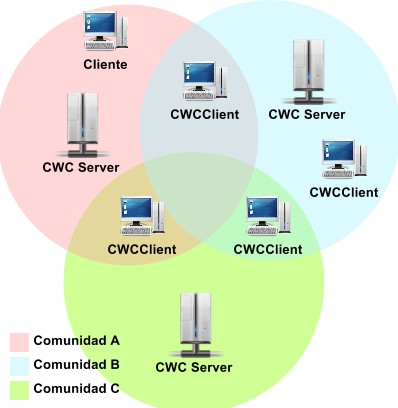
\includegraphics[scale=0.5]{gfx/ComunidadWebCache}
  \caption{Comunidad Web Caché}
  \label{ComunidadWebCache}
\end{figure}

En esta sección se describirá la arquitectura que seguirá cada una de las partes que conforman el CWC.
%----------------------------------------------------------------------------------------

\section{CWC Server}

En la figura \ref{ComunicacionCWCServer}, se puede observar el esquema de una comunicación utilizando CWC, esta comunicación debe ser transparente, de manera que un usuario que no utilice CWC será atendido directamente por el servidor web, en el caso de que un cliente si la utilice entonces esta será atendida por la comunidad  y el servidor. 


\begin{figure}[h]
  \centering
    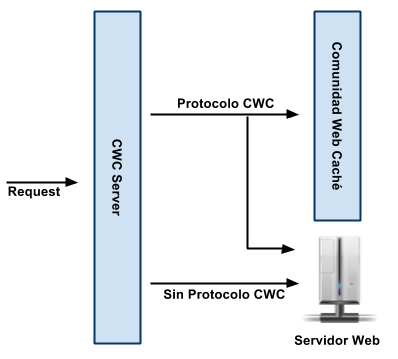
\includegraphics[scale=0.75]{gfx/ComunicacionCWCServer}
  \caption{Comunicación del CWC Server}
  \label{ComunicacionCWCServer}
\end{figure}


Por otro lado, como se puede observar en la figura \ref{ArquitecturaCWCServer}, se presenta una arquitectura multicapa, en los siguientes apartados se explicará cada una de las capas y la interacción entre ellas.

\begin{figure}[h]
  \centering
    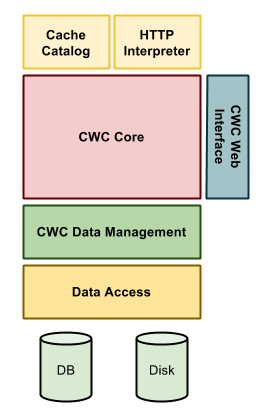
\includegraphics[scale=0.75]{gfx/ArquitecturaCWCServer}
  \caption{Arquitectura CWC Server}
  \label{ArquitecturaCWCServer}
\end{figure}

%------------------------------------------------

\subsection{Data Access}

La capa de acceso a datos implementa toda la lógica para realizar el acceso a datos en este caso se deberá implementar para el acceso para:

\begin{enumerate}
\item Base de datos: En el caso de la base de datos, este será el repositorio donde se almacenarán las estadísticas y la información de los objetos y los miembros de la CWC.
\item Disco: En este caso se trata de archivos planos de texto, de acceso secuencial que se utilizarán para almacenar logs de acceso, logs del CWC Server en general. Los logs de acceso serán analizados una vez a la semana y se almacenarán en la base de datos. Este proceso no se realiza de forma continua pues es necesario reducir el tráfico al disco y utilizar la mínima cantidad de recursos.
\end{enumerate}

%------------------------------------------------

\subsection{CWC Data Management}

El CWC Data Management, actuará como una caché para la base de datos, contendrá la información que se está utilizando  de la base de datos actualmente, más la información que se está generando por el uso del sistema. Las estructuras permanecerán en memoria y actuarán como si fuesen la capa de acceso a datos, pero en realidad todo se estará trabajando desde la  memoria. 

Periódicamente se realizará una descarga de toda esta información hacia la base de datos. La justificación para hacerlo de esta manera es para disminuir la cantidad de accesos a la base de datos y tener la información requerida en memoria para ser accedida de manera rápida y reducir el gasto adicional debido al uso de CWC. En lo referente a logs, éstos ingresarán directamente a disco, pues esta información es de solo lectura y no será analizada en tiempo real para tomar decisiones. 

El tiempo entre cada descarga será definido por el administrador del sitio web, hay que tomar en cuenta que debido a que esta información se va a mantener en memoria volátil, ésta se puede perder, pero este es un riesgo que se asumirá en favor de brindar un mejor servicio. 

Debido a que el periodo de tiempo entre cada descarga es configurable, si se desea reducir el riesgo de perder información, este tiempo deberá tender a ser corto, de lo contrario, puede ser tan largo como se desee. 


%----------------------------------------------------------------------------------------

\subsection{CWC Core}

En la capa CWC Core es donde se implementa toda la funcionalidad de la Comunidad Web Caché, en esta capa se implementará:

\begin{itemize}
\item Administración de Objetos Cachéables.
\item Administración de miembros de la CWC.
\item Administración de estadísticas.
\item Se contará con un módulo para toma de decisiones en base a las estadísticas recolectadas.
\item Comunicación con el servidor web.
\item Comunicación con los miembros de las cachés.
\end{itemize}

La capa CWC Core implementará toda la funcionalidad fundamental de la Comunidad Web Caché, ésta tendrá interacción con:
\begin{itemize}
\item La capa CWC Data Management para escribir y leer datos.
\item La capa CWC Web Interface para comunicarse con el servicio web.
\item La capa CWC HTTP Interpreter para recibir las peticiones, analizarlas y determinar si éstas son válidas y utilizan el Protocolo CWC. Además enviará mensajes utilizando el este mismo protocolo.
\item La capa CWC Caché Catalog para comunicarse con las cachés, para recibir y enviar mensajes con estas, tendrá una conexión permanente con éstas para realizar la comunicación.
\end{itemize}

\subsection{CWC Cachés Catalog}
Esta capa es la que se encarga de tener una conexión permanente con las cachés y también de intercambiar cualquier mensaje con éstas, es el módulo que se comunica a través del protocolo CWC, está constantemente intercambiando mensajes con las cachés para recolectar estadísticas, para indicar cambios de estados en los objetos, entre otros. 

\subsection{CWC Protocol Interpreter}
En esta capa se realiza el análisis de cualquier petición utilizando el protocolo HTTP,  se identifica si la petición utiliza correctamente el protocolo CWC, si es así se pasa el mensaje a la capa CWC Core para que sea atendida. Cuando su atención termine recibirá la respuesta y la enviará al cliente que realizó la petición, en el caso de que la petición no utilice el protocolo CWC será enviada al CWC Web Interface que actuará como un simple puente hacia el servidor web.

\subsection{CWC Web Interface}
Como se ha mencionado anteriormente, el CWC Server se implementará como un módulo de un servidor web existente. 

Este módulo será una capa que actuará como un interfaz para intercambiar datos con las estructuras internas del servicio web y para reenviar las solicitudes que deban ser atendidas por éste.

\section{CWC Client}
En la figura \ref{ComunicacionCWCClient} se muestra el esquema general del mecanismo de comunicación del CWC Client. Este actuará como un "proxy web caché" para las peticiones que envía el cliente. 

Por ejemplo, si se envía una petición a http://www.cwc.com esta petición será interceptada por el CWC Client y resuelta mediante el protcolo CWC, al final el CWC Client se encarga de obtener el archivo desde las diferentes cachés y ensamblarlo, además también se ocupa de servirlo al navegador web. El uso de una Comunidad Web Caché es totalmente trasparente para el usuario y el navegador web. Una versión más detallada de lo que sucede es la siguiente:

\begin{enumerate}
\item El CWC Client, intercepta la petición.
\item Se verifica que el Servidor Web utilice el protocolo CWC.
\item En el caso de que no se utilice, se realizará la petición directamente al servidor.
\item En el caso de que se utilice, se solicitará la lista de cachés con el objeto al servidor.
\item Se inicia la descarga distribuida.
\item Se vuelve a ensamblar el archivo una vez que se tengan todas las partes.
\item Se envía el resultado al navegador web.
\end{enumerate}

\begin{figure}
  \centering
    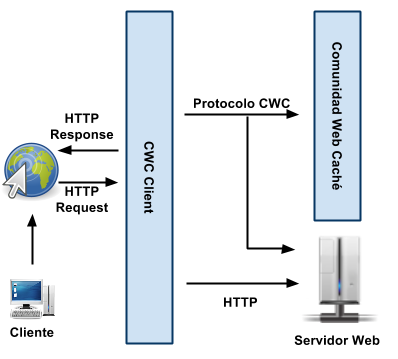
\includegraphics[scale=0.75]{gfx/ComunicacionCWCClient}
  \caption{Comunicación del CWC Client}
  \label{ComunicacionCWCClient}
\end{figure}

La arquitectura del CWC Client es muy similar al de CWC Server. En la figura \ref{ArquitecturaCWCClient} se muestra una descripción gráfica, donde las principales diferencias radican en:

\begin{enumerate}
\item No cuenta con una base de datos.
\item No cuenta con un servidor web. 
\item Funcionará como una extensión para el navegador web. 
\end{enumerate}

\begin{figure}
  \centering
    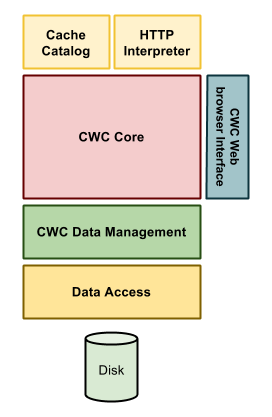
\includegraphics[scale=0.75]{gfx/ArquitecturaCWCClient}
  \caption{Arquitectura CWC Client}
  \label{ArquitecturaCWCClient}
\end{figure}

\subsection{Data Access}
En esta capa se implementará toda la lógica para el acceso a datos, en este caso solo se realizarán accesos a disco, por lo mencionado anteriormente, pues no cuenta con una base de datos del lado del cliente y además porque la principal funcionalidad de ésta es realizar la transmisión de archivos a disco. 

\subsection{CWC Data Management}
Esta capa también como en el CWC Server, funciona como una caché de los datos, esto para reducir los accesos a disco que son sumamente costos.
En caso que un archivo sea leído desde multiples localizaciones, éste acceso se agilizará a través un la memoria de acceso aleatoria (RAM).

\subsection{CWC Client Core}
La capa CWC Client Core, implementará toda la funcionalidad básica de la Comunidad Web Caché, como lo es:

\begin{enumerate}
\item Interacción con el navegador web o agente de usuario.
\item Administración de la caché.
\item Verificación de Consistencia.
\item Administración de la membresía a la comunidad.
\item Servir un archivo.
\end{enumerate}

\subsection{CWC Caché Catalog}
Esta capa implementa el protocolo CWC en forma pura, cuando se trata de una caché, ésta capa se encarga de realizar toda la comunicación entre la caché y el servidor, mantiene una conexión con el servidor e intercambia mensajes. 

\subsection{CWC HTTP Interpreter}
Esta capa implementa de manera muy básica el protocolo HTTP, sirve como cliente para hacer los HTTP Distributed Get y para servir partes de archivos. Además sus funciones son:
\begin{enumerate}
\item Realizar las peticiones HTTP.
\item Servir Archivos.
\end{enumerate}

\subsection{CWC Web Browser Interface}
Esta se encarga de integrarse con la arquitectura del navegador web o el agente de usuario, en este caso se integra para capturar todas las peticiones HTTP y enviarlas en formato CWC. % Chapter 9 - Rendimiento
% Chapter 10

\chapter{Diseño del CWC} % Chapter title

\label{ch:diseno_cwc} % For referencing the chapter elsewhere, use \autoref{ch:name} 

CWC es un modelo de web caching distribuido, el cual busca hacer un uso eficiente de los recursos computacionales disponibles tanto en el servidor como en los clientes mediante el establecimiento de una comunidad. Esta comunidad tiene como objetivo que los clientes proporcionen una cantidad finita de recursos para establecer una Web Caché Distribuida la cual permita reducir el tráfico sobre el servidor, ya que los archivos serán servidos desde múltiples localizaciones y en una mayoría de casos, sin trabajo adicional por parte del servidor, más que indicar donde se encuentra el archivo y como accederlo. 

Con el establecimiento de la Web Caché Distribuida y al reducir el tráfico sobre el servidor, se permitirá atender a más clientes y hacer la comunidad mucho más grande. Lo cual, en última instancia, implica una Web Caché Distribuida mucho más grande y con más recursos.
%----------------------------------------------------------------------------------------

\section{CWC Server}

El CWC Server es una aplicación que se Integra con el servidor web, su función consiste en realizar la administración de la CWC e interceptar las peticiones de los clientes que utilizan CWC. Entre las funciones del CWC Server se encuentran: 

\begin{itemize}
\item Administración del Caché local
\item Administración del CWC
\item Estadísticas
\item Segmentación de Archivos
\item Administración Remota de Caché
\end{itemize}

%------------------------------------------------

\subsection{Administración de Objetos en la Caché local}

En un servidor web existen gran cantidad de objetos, que van desde los documentos HTML y CSS más comunes hasta lo que hoy conocemos como multimedia, que incluye un gran número de archivos de gran tamaño como video y música. Además también existen de aplicaciones de tiempo real como videoconferencias y streaming de video y audio. La administración de Objetos en la caché local se refiere a cómo identificar cuáles objetos se pueden agregar a la caché del CWC y cuales no. Cada objeto contará con los siguientes atributos:

\begin{itemize}
\item \textit{Checksum}: Esto con el objetivo de saber si el archivo esta corrupto. No se hablará del cálculo del Checksum.
\item \textit{Id}: El archivo tendrá su identificador único, generado automáticamente.
\item \textit{Localización}: URI relativo al URL del sitio web.
\item \textit{Cachés}: Cuáles clientes CWC poseen una copia de este objeto. 
\item \textit{En Caché}: Bandera que indica si el objeto puede ser compartirse a través del CWC o no.
\item \textit{Tiempo expiración}: Dentro de cuanto el objeto será obsoleto. 
\end{itemize}

Todos estos atributos, excepto uno, deben de perdurar en disco, para evitar fallas eléctricas o bien el apagado del equipo. El atributo \textit{Cachés} será mantenido en memoria, pues es un dato que se calcula en tiempo de ejecución de la CWC.

A continuación se presentan las acciones presentes en la Administración de Objetos en la Caché local:

\begin{description}

\item[Agregar un nuevo Objeto] Cuando se agrega un nuevo objeto al servidor web se deben calcular sus atributos y almacenarlos. Cuando una nueva caché obtiene un objeto se actualiza su información de cachés, lo cual quiere decir que este objeto puede ser servido desde una caché más.

\item [Modificar un Objeto] Existen dos tipos de modificaciones: 
	\begin{description}
	\item[Soft] Una modificación soft no implica que la caché tenga que volver a obtener el objeto, una modificación soft es cambiar la localización del archivo, cambiar las cachés del archivo, cambiar el estado de Cacheable, cambiar su tiempo de expiración.
	\item [Hard] La modificación hard, se refiere al cambio del tamaño del archivo lo cual implica un cambio de su Checksum.

Cada atributo implica diferentes que deben ser tomadas, entre estas se tiene:

		\begin{itemize}
		\item \textit{Checksum y Tamaño}: Al darse un cambio en estos atributos se deben invalidar todas las cachés de este objeto y notificar a las mismas para que borren sus copias y si es necesario que obtengan una copia fresca.
		\item \textit{Id}: No se hacen cambios de Id.
		\item \textit{Localización}: tiempo de expiración y Cachés: Simplemente se actualiza la información no se notifica a las cachés.
		\item \textit{En Caché}: Se notifica a las cachés el nuevo estado para que invaliden y borren su copia.
		\end{itemize}

\end{description}

\item [Borrar un Objeto] Cuando se borra un objeto, se borra el objeto junto con sus atributos y además se notifica a las cachés para que borren su copia.

\item [Verificar Expiración] El CWC Server deberá estar revisando si los objetos de la caché se encuentran válidos, en el caso de que alguno sea inválido se establece el objeto como no-cacheable y se trata como una modificación. 

\item [En Transferencia] Si se da una modificación hard o un borrado mientra el objeto se está transfiriendo, como política se deben invalidar todas las copias incluyendo la original y borrarlas hasta que se termine de servir a todos los clientes que están recibiendo el archivo.

\end{description}

%------------------------------------------------

\subsection{Administración del CWC}

Esta administración es muy relativa ya que no se tendrá control completo sobre ésta, en este caso nos referimos a los clientes que conforman la comunidad y a los objetos que pueden ser compartidos en la caché.

Cuando el CWC Server se inicia por primera vez, posee una caché que vamos a definir como \textit{fría}, lo cual quiere decir que no existen miembros en la comunidad y por ende no existen objetos cachéados. Las acciones que se pueden dar son las siguientes:

\begin{description}
\item[Agregar un nuevo miembro] Cuando se agrega un miembro se crea en memoria la estructura para este cliente y se establecen los recursos aportados por este cliente, dentro de la información importante que se debe almacenar, se encuentra:
	\begin{itemize}
	\item Los clientes que está sirviendo.
	\item Los archivos que tiene en su caché.
	\item La localización geográfica 
	\item El estado del caché: Activa/Inactiva.
	\item El estado del cliente: online/offline.
	\end{itemize}
	
\item [Agregar un miembro existente] Se puede haber dado el caso que el servidor fallase, por lo que la información de las cachés se perdería. O bien, que alguna de las cachés fallara y se perdiera la conexión con el servidor. Esto último implicaría que la caché quedase en un estado offline, o se desactivará. Para agregar una caché existente sería necesario:

	\begin{enumerate}
	\item La caché se comunica con el servidor, ya sea porque se recuperó de alguna falla o se activó de nuevo o porque el servidor fue el que falló y ya se encuentra en línea de nuevo.
	\item El servidor busca en su lista para ver si la caché se encuentra disponible.
	\item En el caso de que se encuentre:

		\begin{enumerate}
		\item Se le envía la lista de archivo que debería tener cachéados y su respectivo Checksum.
		\item La caché verifica que tiene los archivos y que son correctos.
		\item Si todo está bien la caché confirma para ser promovida a online.
		\item Si algún archivo esta corrupto o no existe, se borra y se envía la invalidación al servidor.
		\item Se confirma el estado consistente para ser promovida a online.
		\end{enumerate}	
	
	\item En el caso de que no se encuentre:
		\begin{enumerate}
		\item Se le solicita una lista de archivos cachéados y su Checksum.
		\item Cuando la caché los envía, se verifican los archivos y su Checksum.
		\item Si todo está bien se confirma su estado online al crear las estructuras del miembro con sus atributos.
		\item Si alguna archivo fue borrado, modifica o esta corrupto, se indica que se invalida y una vez que se confirma la invalidación se crean las estructuras del miembro y se le notifica a la caché que esta online.
		\end{enumerate}	
	
	\end{enumerate}
	
\item [Modificar un miembro] Cualquiera de los atributos de un miembro se puede modificar, lo más importante es conocer si éste está activo/no activo, esto se logra mediante la  revisión periódica del estado de las cachés.

\end{description}

%----------------------------------------------------------------------------------------

\subsection{Estadísticas}

En una comunidad al igual que en cualquiera, hay diversidad de miembros, algunos cuentan con muchos recursos, otros con pocos o algunos fallan bajo presión. La idea con las estadísticas, es que una vez que se solicita un objeto, enviar la lista de cachés que lo tienen disponible, ordenada de tal manera que se presenten los que históricamente tiene mejores referencias de primero. 

Esto no quiere decir que a los que tienen un bajo historial se dejarán fuera, sino que cuando se deba atender una petición tendrán menor trabajo que el resto. Tampoco quiere decir que se quedarán haciendo el peor trabajo siempre, sino más bien, se pretende implementar un sistema de puntos en el cual, presente la oportunidad de crecer en confianza y convertirse en una de las cachés más altas en el ranking.

Entre las estadísticas que se van a recolectar son:

\begin{description}
\item[Logs de Acceso] Se debe llevar un recuento para cada petición, de quien la atendió y tiempo de respuesta.

\item[Bookkeeping] Para cada una de las cachés se debe tener un histórico de:
	\begin{itemize}
	\item Tiempo de respuesta.
	\item Número de clientes atendidos por unidad de tiempo.
	\item Número de veces que ha fallado.
	\item Velocidades de trasferencia mínimas y máximas.
	\item Archivos en caché y número de veces que han sido trasmitidos.
	\end{itemize}
	
\item[Sistema de Puntos] El sistema de puntos funcionará de la siguiente manera:

	\begin{description}
	\item[Puntos estáticos] Estos puntos son dados en el transcurso normal de la vida del CWC.
		\begin{itemize}
		\item La máxima cantidad de puntos es 100 y la mínima es -100.
		\item  Un miembro nuevo, recibirá una bonificación de 50 puntos por formar parte de CWC.
		\item Cada 6 horas que el miembro permanezca online, recibirá una bonificación de 1 punto con un máximo de 4 puntos diarios. En el caso contrario perderá un punto cada 6 horas con un máximo de 4 diarios.
		\item  Si el miembro se desactivó, perderá un punto cada 12 horas por estar inactivo. Con un máximo de 2 puntos diarios.
		\item Por cada cliente atendido satisfactoriamente el miembro recibirá un total de 2 puntos, por cliente atendido insatisfactoriamente el miembro perderá 3 puntos.
		\end{itemize}
		 
	\item[Bonificaciones] Las bonificaciones son dadas por acciones extras beneficiosas hacia los clientes. 
	
		\begin{itemize}
		\item El miembro de la caché con el mejor tiempo de respuesta ganará una bonificación de 10 puntos.
		\item Los miembros de la caché con tiempo de respuesta mayor a la media ganará	n un punto adicional.
		\item El miembro de la caché que haya transmitido el mayor número de veces el  objeto solicitado, recibirá un bono de 10 puntos.
		\end{itemize}

	\item[Cálculo total] A continuación se detallan las reglas que dictan cómo se realizará el cálculo total de los puntos acumulados: 
	
		\begin{enumerate}
		\item Con las reglas y bonificaciones anteriormente mencionadas, se calcula el top de miembros de la caché.
		\item Con el top de miembros listo, se eliminan todos aquellos que están atendiendo a su máximo número de clientes permitido que se calcula mediante: 
		$$ \frac {\text{conexión de subida}}{\text{mínima velocidad para servir archivos}} $$ 
		Esto quiere decir que si se asigna una velocidad mínima para servir archivos de 64Kbps y el miembro de la caché estableció su conexión de subida en 512Kbps, el número máximo de clientes que puede atender simultáneamente es 8.
		\item Para evitar la sobrecarga de trabajo sobre una caché, las cachés recibirán una penalización con base al número de usuarios que están atendiendo, la regla establece que una caché perderá: 
		
		$$ \text{número de clientes actuales} * 3 \text{puntos} $$
		\end{enumerate}
	
	\end{description}

\end{description}


\subsection{Segmentación de Archivos}

Cuando se va a servir un archivo desde la caché, éste se debe descomponer en un número de segmentos. Un posible tamaño de un segmento podría ser 128KB y éste podría corresponder al ancho de banda mínimo de la CWC. 

Por ejemplo, si se desea descargar un archivo de 10MB, se debe de descomponer en partes de 128KB y ésta será la unidad de descarga de la caché. El segmento debe ser establecido por el administrador del sitio web, entre más pequeña mejor.

\subsection{Administración Remota de Caché}

Como se mencionó anteriormente, es posible que el cliente delegue la administración de la caché local al servidor. En el caso, el servidor se encargará de decir cuando se debe tener un archivo en la caché y cuando no se debe. La decisión de retirar un archivo o agregar otro a la caché, toma en cuenta si los archivos están siendo solicitados frecuentemente. Entonces el servidor envía los siguientes mensajes a las cachés:

\begin{itemize}
\item \textit{Agregar Objeto}: Envía el id archivo y la caché se encarga de solicitarlo.
\item \textit{Borrar Objeto}: Envía el id del archivo y la caché se encarga de borrarlo.
\end{itemize}

\section{CWC Client}
El CWC Client es una aplicación que se integra con el navegador web o agente de usuario, la principal función de este es poder obtener archivos de la CWC.  Entre las funciones del CWC Client se encuentran:

\begin{itemize}
\item Asociación a la comunidad
\item Administración de la Caché local
\item Otras funciones de administración
\end{itemize}

\subsection{Asociación a la comunidad}

Existen dos formas diferentes para formar parte de la comunidad:

\begin{description}
\item[Contribuyente] Funciona de la siguiente manera: el usuario instala la aplicación CWC Client e inicia la navegación por diferentes páginas. Cuando se encuentra un servidor que soporta el protocolo CWC y se solicita un objeto que se pueda compartir en la caché de CWC, el cliente empieza a formar parte de la comunidad (si tiene instalado CWC Client es porque se desean compartir los recursos) con los parámetros mínimos, se podría decir que obtiene una membresía mínima.

\item[Activa] En este caso, el usuario quiere ser miembro de la CWC de un sitio en específico. Por lo que el usuario crea de manera específica la membresía y establece los recursos que desea compartir.

La diferencia radica en que si el usuario se convierte en miembro de manera voluntaria, la administración de la caché será realizada por el servidor. En todo caso, si la membresía es activa se puede cambiar a contribuyente.

Se puede dar el caso de que no desee formar parte de la comunidad de algún sitio en específico, entonces se puede configurar CWC Client de manera que ignore los sitios de una lista negra.

Para dejar de ser un miembro de la caché, se debe:

\begin{itemize}
\item Indicar que no se quiere pertenecer más a esta (Agregarla a la lista negra).
\item No poseer ningún archivo de en caché (involuntaria).
\end{itemize}

\end{description}


\subsection{Administración de la Caché Local}

La administración de la caché se puede dar de 3 formas, atendida por el cliente, desatendida (por defecto cuando la membresía es de tipo contribuyente) y por último administrada por el servidor (solo se utiliza cuando la membresía es activa):

\begin{description}
\item[Desatendida] En este caso, cuando la caché está llena, la misma caché escoge el archivo menos solicitado y lo borra, así sucesivamente hasta que se libera suficiente espacio como para almacenar el archivo. 
\item[Atendida] El usuario puede borrar archivos de la caché a su gusto. Para ello tendrá una interfaz de selección de archivos que se encuentren en la caché.
\item[Manejada por el Servidor] El servidor por si solo decidirá cuáles archivos deben estar en caché y cuáles no, sus decisiones serán transmitidas a la caché mediante el envío de mensajes. 
\end{description}


\subsection{Otras Funciones de Administración}
Otras funciones de administración que posee el CWC Client son las siguientes:
\begin{description}
\item[Invalidar contenido] Si se recibe un mensaje de que el contenido está inválido, automáticamente se borra el objeto y se descarga.

\item [Revisión de Consistencia] Periódicamente se verifica si los contenidos de la caché son correctos, se le solicita al servidor el Checksum para los archivos que se encuentran en la caché y se comparan. Si están bien perfecto si no se procede a hacer una invalidación de contenido.

\item [El servidor está vivo] Revisión constante del servidor, se debe establecer si se encuentra funcional o está fuera de línea.

\item [Mensaje de Offline, activo o desactivo] En cualquiera de estos casos la caché se comunica con el servidor para indicarle su nuevo estado.

\item [Transferencia de estadísticas] Periódicamente el cliente envía las estadísticas que se han producido con respecto a los objetos que se encuentran en su caché. 

\item [Agregar contenido a la caché] Es una acción ejecutada en el caso que se envíe la petición por parte del servidor o porque se ingrese a algún servidor web que utiliza CWC.
\end{description}
 % Chapter 10 - Análisis y Resultados

\part{Conclusiones} % Second part of the thesis
% Chapter 11

\chapter{Metodología} % Chapter title

\label{ch:metodologia} % For referencing the chapter elsewhere, use \autoref{ch:name} 

Como parte de la metodología del presente proyecto se discutirán herramientas que permitirán realizar la medición de la eficiencia, en relación a la transferencia de información entre los clientes y un servidor. Esta medición se realizará en un ambiente definido en las siguientes secciones y además se creará una comparación entre el protocolo HTTP y un prototipo del protocolo CWC. 

Por otro lado como parte del análisis de costos se establecerá los requerimientos mínimos necesarios, para poder desarrollar los ambientes de pruebas. Ésta configuración de hardware conformará los parámetros para el cálculo de costo. 

%----------------------------------------------------------------------------------------

\section{Herramientas}

%------------------------------------------------

\subsection{httperf}

Httperf es una herramienta para medir el rendimiento de aplicaciones web. Provee una manera flexibe de generar múltiples cargas de trabajo utilizando HTTP y con ellas poder medir el rendimiento Web. Puede observarse el funcionamiento de esta herramienta en la figura \ref{httperf}.

\begin{figure}[h]
  \centering
    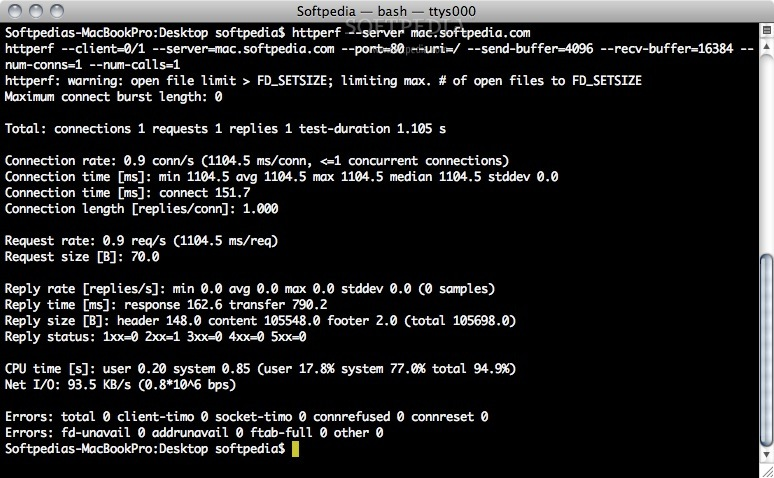
\includegraphics[scale=0.4]{gfx/httperf}
  \caption{Funcionamiento de httperf}
  \label{httperf}
\end{figure}

\subsection{OpenWebLoad}
OpenWebLoad es otra herramienta muy sencilla pero poderosa, es completamente en consola y permite hacer peticiones de archivos. Dentro de la información que arroja está el número de ejecuciones, tiempo de respuesta de cada ejecución y tiempo de ejecución promedio. Puede observarse el funcionamiento de esta herramienta en la figura \ref{OpenWebLoad}.

\begin{figure}[h]
  \centering
    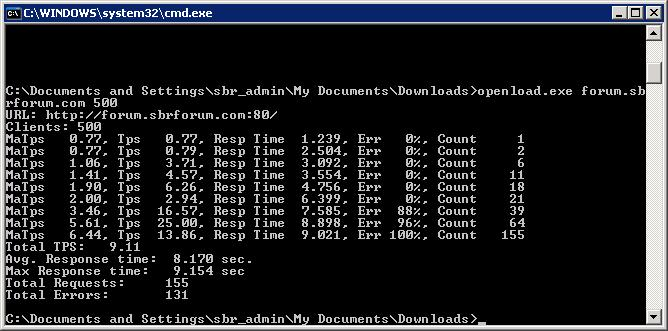
\includegraphics[scale=0.6]{gfx/OpenWebLoad}
  \caption{Funcionamiento de OpenWebLoad}
  \label{OpenWebLoad}
\end{figure}

\subsection{Time}
\label{subsec:time}
El comando time puede servir para obtener el tiempo que tarda una aplicación en completarse. En este caso se puede combinar con cualquier otra aplicación, por ejemplo con el prototipo del CWC. Puede observarse el funcionamiento de esta herramienta en la figura \ref{time}.

\begin{figure}[h]
  \centering
    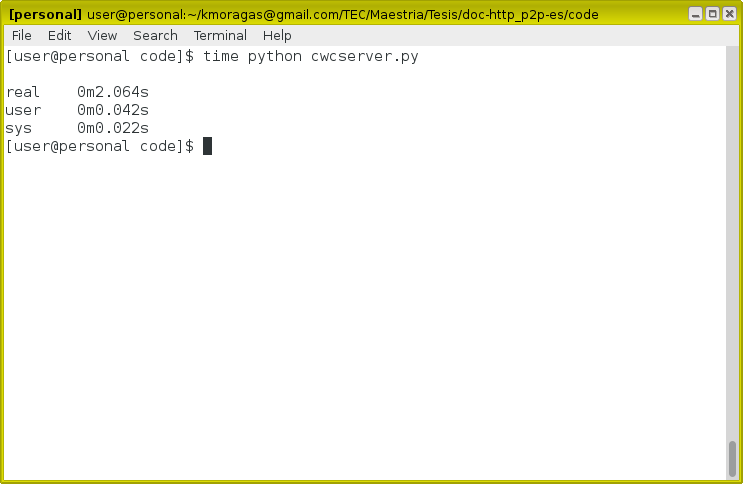
\includegraphics[scale=0.6]{gfx/time}
  \caption{Funcionamiento de time}
  \label{time}
\end{figure}

%------------------------------------------------

\subsection{JMeter}

JMeter forma del proyecto TomCat y es una herramienta muy utilizada para realizar pruebas de carga en un sitio web, mediante esta herramienta se puede describir prácticamente todo el comportamiento de un usuario dentro de un sitio web, desde cuando se autentica hasta cuando se llenan campos de texto en un formulario. Puede observarse el funcionamiento de esta herramienta en la figura \ref{jmeter}.

\begin{figure}[h]
  \centering
    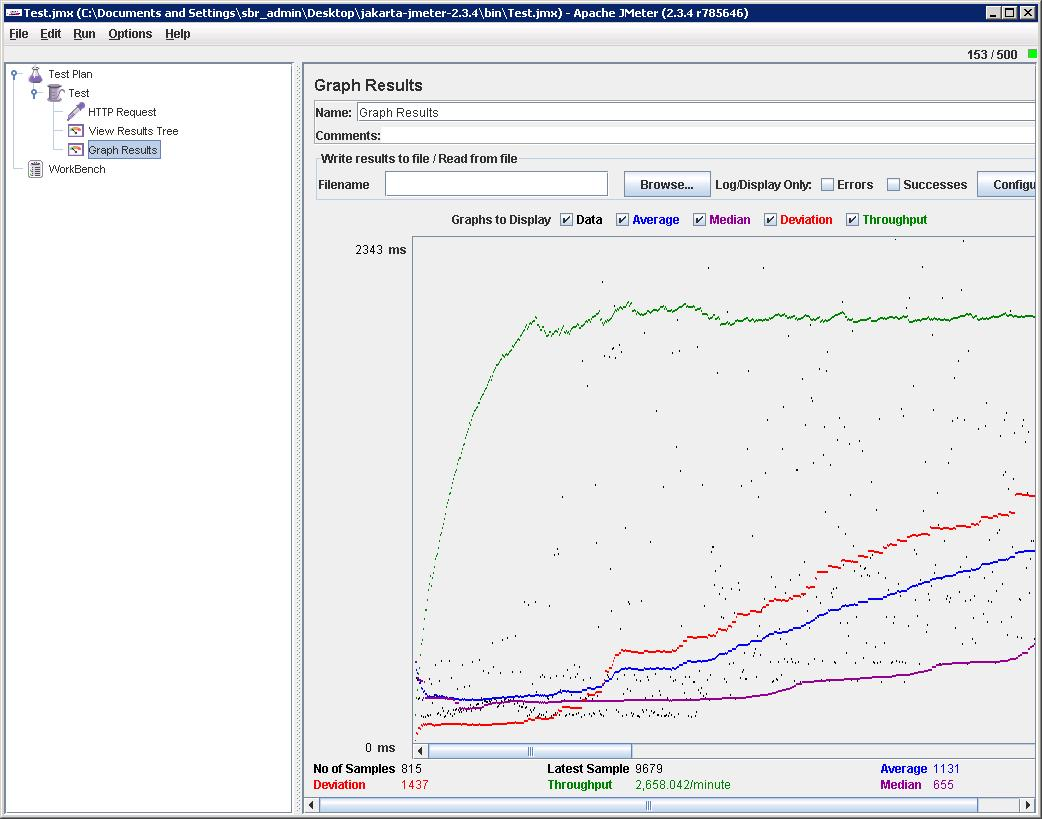
\includegraphics[scale=0.4]{gfx/jmeter}
  \caption{Resultados de Tiempo de Respuesta}
  \label{jmeter}
\end{figure}



%----------------------------------------------------------------------------------------

\section{Parámetros de las pruebas}
\label{sec:parametros_pruebas}

\subsection{Servidor Web y Servidor Caché}
\label{subsec:servidor_web}
El servidor web que utilizará será Apache. En relación a la presente metodología, la configuración en hardware para los casos de prueba será:

\begin{itemize}
\item GNU/Linux Debian Wheezy.
\item Apche2.2 con la instalación por defecto.
\item 4GB de RAM 
\item Dos núcleos
\item Al menos 100MB de espacio disponible.
\item Una interfaz de red.
\end{itemize}

Para determinar los valores de la configuración se basó en los recursos mínimos que se pueden adquirir a través de un sitio común de venta de dispositivos electrónicos. 

\subsection{Tipos de archivos de prueba}
\label{subsec:archivos}
En este caso se utilizarán archivos de diferente tipo y de diferente tamaño para realizar las pruebas, entre los tipos de archivos que se utilizarán son:

\begin{itemize}
\item Imágenes JPEG, PNG y GIF
\item Videos FLV, mpeg y AVI
\item Documentos ODT, DOC y XSLT
\item Instaladores EXE, BIN, MSI, DEB, RPM
\end{itemize}

Los tamaños de los archivos variarán, el máximo tamaño deberá ser de 600MB y el mínimo de de 1MB.

\subsection{Estrategia de las pruebas}
\label{subsec:estrategia_pruebas}
Como parte de la estrategia se limitará el ancho de banda a 200 KB/s en cada servidor. Además las pruebas que se deben ejecutar son:

\begin{itemize}
\item Con archivos pequeños, tamaños menores a los 100MB.
\item Archivos Grandes, tamaños superiores a 100MB.
\item Por tipo de archivo.
\item Todos los archivos.
\end{itemize}

\section{Escenarios}
\label{sec:escenarios}

\begin{description}
\item[Sin Web Caché] Este es el modelo tradicional de HTTP en el cual se tiene un sólo servidor web y múltiples clientes se conecta a él. En el caso de la prueba se configurará confirme a lo definido en la sección \ref{subsec:servidor_web}, además se configurará un límite de transferencia entre el servidor y el cliente definido en la sección de estrategia de pruebas ubicada en el apartado \ref{subsec:estrategia_pruebas}. Por otro lado, este servidor servirá los archivos definidos en la sección \ref{subsec:archivos}.

\item [Prototipo de CWC] Se medirá el comportamiento de la transferencia a través del prototipo de CWC. Los archivos a medir son igualmente los definidos en la sección  \ref{subsec:archivos}. Por otro lado la configuración de hardware por cada nodo será la misma que se presenta en la sección \ref{subsec:servidor_web}, pero en éste caso no será necesario configurar ningún servidor web en el sistema. También se limitará el ancho de banda entre los nodos y el cliente.
\end{description}
 % Chapter 11 - Conclusiones y Trabajo Futuro

%----------------------------------------------------------------------------------------
%	THESIS CONTENT - APPENDICES
%----------------------------------------------------------------------------------------

\appendix

\part{Appendix} % New part of the thesis for the appendix

% Appendix A

\chapter{Appendix Test}

%----------------------------------------------------------------------------------------

\lipsum[13-14]

%----------------------------------------------------------------------------------------

\section{Appendix Section Test}
\lipsum[15]

\graffito{More dummy text}
\lipsum[16]

%----------------------------------------------------------------------------------------

\section{Another Appendix Section Test}
\lipsum[17]

\begin{table}
\myfloatalign
\begin{tabularx}{\textwidth}{Xll} \toprule
\tableheadline{labitur bonorum pri no} & \tableheadline{que vista}
& \tableheadline{human} \\ \midrule
fastidii ea ius & germano &  demonstratea \\
suscipit instructior & titulo & personas \\
\midrule
quaestio philosophia & facto & demonstrated \\
\bottomrule
\end{tabularx}
\caption[Autem usu id]{Autem usu id.}
\label{tab:moreexample}
\end{table}

\lipsum[18]

\begin{lstlisting}[float,caption=A floating example]
for i:=maxint to 0 do
begin
{ do nothing }
end;
\end{lstlisting} % Appendix A
%% Appendix X

\chapter{Appendix Title}

%----------------------------------------------------------------------------------------

% Content begins here % Appendix B - empty template

%----------------------------------------------------------------------------------------
%	POST-CONTENT THESIS PAGES
%----------------------------------------------------------------------------------------

\cleardoublepage% Bibliography

\label{app:bibliography} % Reference the bibliography elsewhere with \autoref{app:bibliography}

\manualmark
\markboth{\spacedlowsmallcaps{\bibname}}{\spacedlowsmallcaps{\bibname}} 
\refstepcounter{dummy}

\addtocontents{toc}{\protect\vspace{\beforebibskip}} % Place the bibliography slightly below the rest of the document content in the table of contents
\addcontentsline{toc}{chapter}{\tocEntry{\bibname}}

\bibliographystyle{plainnat}

\bibliography{Bibliography} % Bibliography

\cleardoublepage% Colophon (a brief description of publication or production notes relevant to the edition)

\pagestyle{empty}

\hfill

\vfill

\pdfbookmark[0]{Colophon}{colophon}

\section*{Colophon}

Este documento utiliza el conjunto de tipografías de \texttt{classicthesis} desarrollado por Andr\'e Miede. El estilo fue inspirado en la tipografía del libro de Robert Bringhurst ``\emph{The Elements of Typographic Style}''

\noindent Esta tesis fue impresa en San José, Costa Rica. Una copia de ella se puede encontrar en la siguiente dirección:

\begin{center}
\url{http://www.kmoragas.com/}
\end{center}
 
\bigskip

\noindent\finalVersionString % Colophon

\cleardoublepage% Declaration

\refstepcounter{dummy}
\pdfbookmark[0]{Declaration}{declaration} % Bookmark name visible in a PDF viewer

\chapter*{Declaration} % Declaration section text

\thispagestyle{empty}

Put your declaration here.
\bigskip
 
\noindent\textit{\myLocation, \myTime}

\smallskip

\begin{flushright}
\begin{tabular}{m{5cm}}
\\ \hline
\centering\myName, \today \\
\end{tabular}
\end{flushright} % Declaration

%----------------------------------------------------------------------------------------

\end{document}